\section{補正理論}
作用力測定装置から得た抗力方向および揚力方向における出力電圧$V_D$,$V_L$を
水槽座標系の$x$軸方向および$y$軸方向の荷重$F_x$,$F_y$に換算する際に,
出力電圧$V_D$,$V_L$と$F_x$,$F_y$の関係性を明らかにするための校正実験を
行う必要がある.
校正実験によって得られた結果を用いて関係性を明らかにするための校正理論について述べる.

\subsection{作用力測定装置と校正実験装置の関係}
はじめに,作用力測定装置と校正実験装置の関係について説明する.
作用力測定装置と校正実験装置の設置位置によって校正実験結果は大きく変動するため,
その影響を考慮し,補正処理を行う必要がある.
このとき以下のような要因が,校正実験結果への影響を与えていると考えられる.

\begin{enumerate}[(1)]
  \item 作用力測定装置にひずみセンサが正確に取り付けることが難しい
  \item 作用力測定装置が回流水槽に正確に設置することが難しい
  \item 作用力測定装置と校正装置の回転軸を一致させることが難しい
\end{enumerate}

ここで,水流に対する座標系を水槽座標系 $(x-y)$,
作用力測定装置の座標系を座標系A $(x'-y')$,
校正装置の座標系を座標系B $(x''-y'')$とする.

このとき,(1) 作用力測定装置にひずみセンサを正確に取り付けることが難しいこと,
(2) 作用力測定装置が回流水槽に正確に設置することが難しいことから,
座標系Aは水槽座標系に対して
$x'$軸は$x$軸から$\theta_x$,$y'$軸は$y$軸から$\theta_y$だけ回転している.
このとき,座標系Aにおいて,$x'$と$y'$は直行しない.
また,座標系Bは水槽座標系に対して
$x''$軸は$x$軸から$y$方向に$\Delta x$,
$y''$軸は$y$軸から$x$方向に$\Delta y$だけオフセットを持つ状態となる.
その位置関係の概略図をFig.7に示す.

\begin{figure}[htbp]
  \begin{center}
    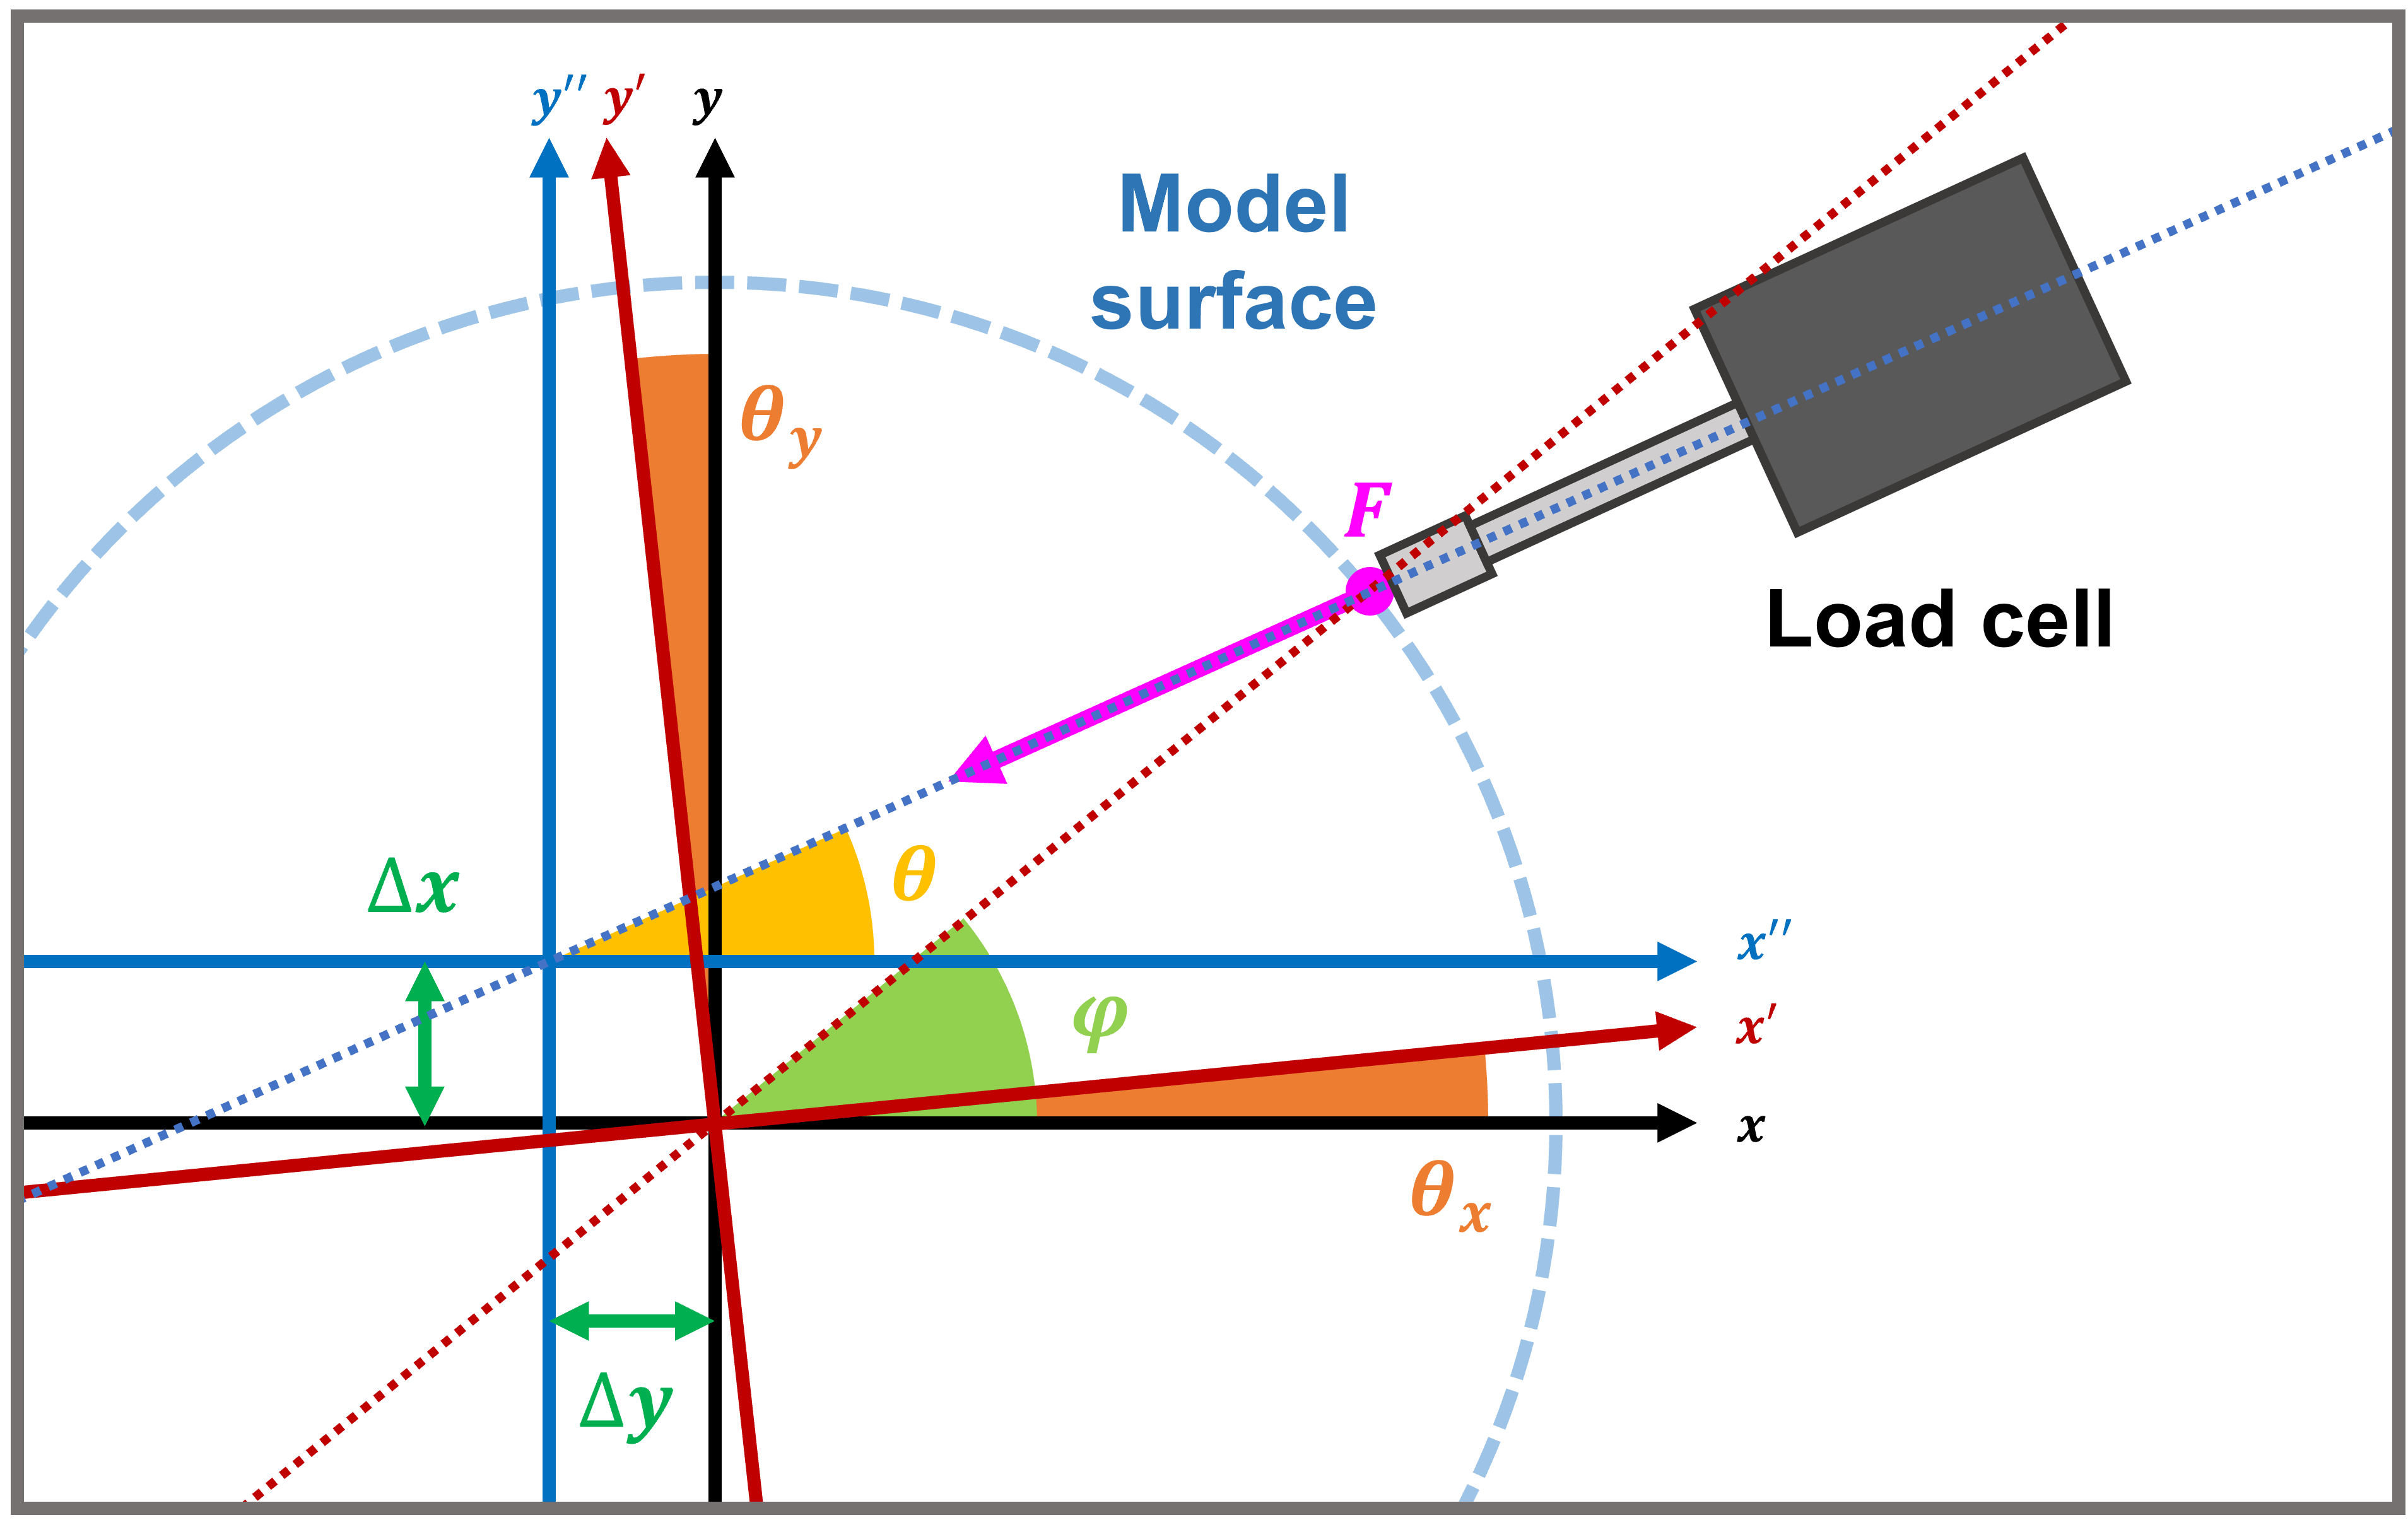
\includegraphics[width=90mm]{images/31-1.png}
    \caption{Coordinate systems relationship}
  \end{center}
\end{figure}

\newpage

\subsection{出力電圧勾配}

作用力測定装置の評価にあたり,作用力測定装置に取り付けられた2組のひずみセンサ
および校正実験の際に作用力を与えるロードセルの出力電圧の対応関係を調べることで評価を行う.
ここで,作用力測定装置において抗力方向のひずみセンサの出力電圧を$V_d$,揚力方向を$V_l$,
ロードセルの出力電圧を$V$とするとき,抗力方向の出力電圧勾配を$v_d$,
揚力方向の出力電圧勾配を$v_l$として以下のように表す.

\begin{align}
  v_d = V_d / V \\
  v_l = V_l / V
\end{align}

また,Fig.7のように座標系を定めるとき,出力電圧勾配の理論値は,
抗力方向を$v_{x\;\mathrm{theory}}$,揚力方向を$v_{y\;\mathrm{theory}}$として,
以下のように与えられる.

\begin{align}
  v_{x\;\mathrm{theory}} & = C \sin\left(\omega t + \frac{3}{2}\pi\right) = C \cos\left(\omega t + \pi
  \right)                                                                                                     \\
  v_{y\;\mathrm{theory}} & = C \sin\left(\omega t + \pi\right) = A \cos\left(\omega t + \frac{1}{2}\pi\right) \\
  C                      & = const \notag
\end{align}

\subsection{補正理論[1] : 座標系の回転における補正理論}

水槽座標系と座標系Aの回転における補正理論を説明する.
ここでは,座標系のオフセットはない($\Delta x = 0$,$\Delta y = 0$)として考える.
上述の通り水槽座標系と座標系Aについて,Fig.8のように回転角$\theta_{x}$,$\theta_{y}$を持つ.
ここで,作用力$F$を与えるとそれぞれの方向に作用力$F_{x}$,$F_{y}$,$F_{x'}$,$F_{y'}$が加わる.
このとき,作用力測定装置から得られる電圧$V_{x'}$,$V_{y'}$は作用力$F_{x'}$,$F_{y'}$に起因するものである.
また,得られた出力電圧$V_{x'}$,$V_{y'}$から,ロードセルの出力電圧$V_1$を用いて
出力電圧勾配$v_{x'}$,$v_{y'}$を求めることができる.
したがって,水槽座標系と座標系Aの関係について,
$v_{x}$と$v_{x'}$および$v_{y}$と$v_{y'}$の関係を明らかにすれば良い,

\begin{figure}[htbp]
  \begin{center}
    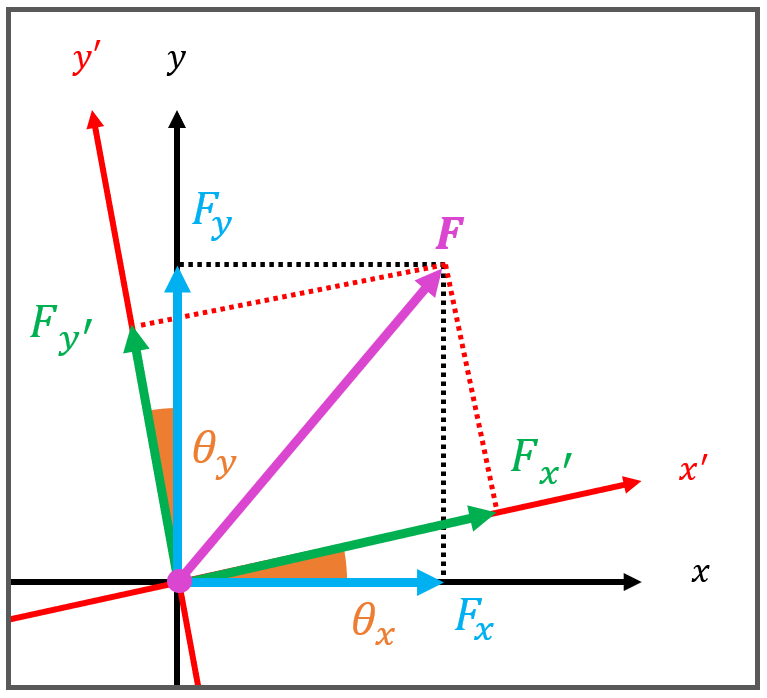
\includegraphics[width=65mm]{images/33-1.png}
    \caption{Relationship between ($x-y$) and ($x'-y'$)}
  \end{center}
\end{figure}

\subsubsection{回転角$\theta_{x}$,$\theta_{y}$の算出}
はじめに,回転角$\theta_{x}$,$\theta_{y}$を算出する.
理論式における$v_{x\;\mathrm{theory}}$及び$v_{y\;\mathrm{theory}}$は正弦波とその位相差で表すことができる.
したがって,校正実験結果の各角度の出力電圧勾配においても同様の正弦波と
その位相差で表すことが可能であると予想することができる.
このとき,離散フーリエ変換を適用し,
波数1の成分について,実部をRe,虚部をImとして
位相角$\phi$を求めることができる.

\begin{align}
  \phi = \arctan \left(\frac{Im}{Re}\right) \cdot \frac{180}{\pi}
\end{align}
\vskip \baselineskip

抗力方向の結果から得られた位相角を$\phi_1$,揚力方向から得られた位相角を$\phi_2$と
するとき,抗力方向の出力電圧勾配$v_d$と
水槽座標系における$x$軸方向の出力電圧勾配の理論値$v_{x\;\mathrm{theory}}$との位相差
$\theta_x$,
揚力方向の出力電圧勾配$v_l$と
水槽座標系における$y$軸方向の出力電圧勾配の理論値$v_{y\;\mathrm{theory}}$との位相差
$\theta_y$を以下のように表される.

\begin{align}
  \theta_x & = \pi - \phi_1           \\
  \theta_y & = \frac{\pi}{2} - \phi_2
\end{align}
\vskip \baselineskip

したがって,$x'$軸,$y'$軸は左回りを正方向として,それぞれ$\theta_x$,$\theta_y$だけ
回転していることとなる.
また,作用力測定装置に取り付けられた抗力・揚力方向のひずみセンサの取付角を$\phi_s$とすると
位相角$\phi_1$,$\phi_2$より求めることができる.

\begin{align}
  \phi_s = \left| \phi_1 - \phi_2 \right|
\end{align}

\newpage

\subsubsection{出力電圧勾配の座標変換}

ここで,水槽座標系と座標系Aについて,Fig.9のように考える.
位相角$\theta_x$,$\theta_y$が求められたことから,
それらを用いて出力電圧勾配の座標変換を行う.
ここで,座標系Aの$x'$軸,$y'$軸を
それぞれ$f_{x}\left(x\right)$,$f_{y}\left(x\right)$として,
水槽座標系の$x$を用いた式で表す.

\begin{figure}[htbp]
  \begin{center}
    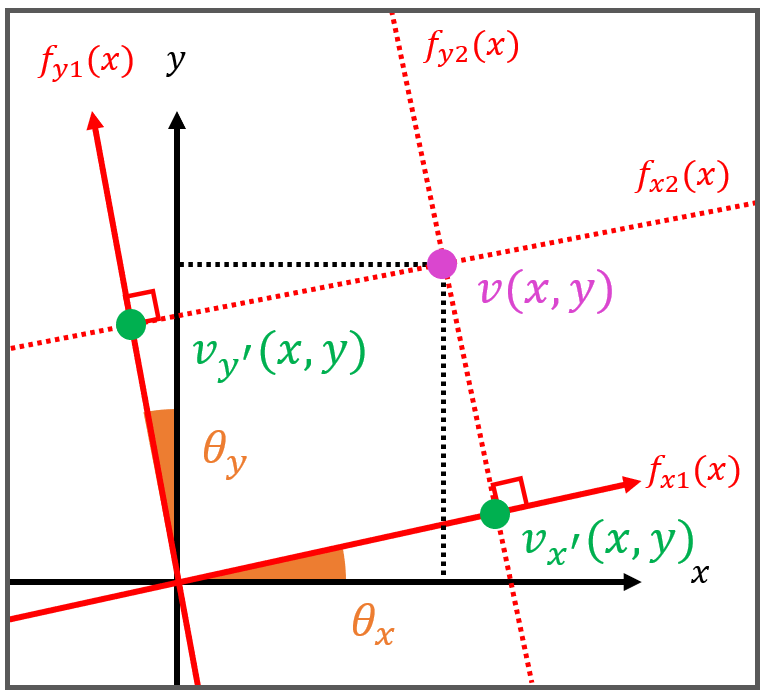
\includegraphics[width=65mm]{images/33-2.png}
    \caption{Coordinate calculation}
  \end{center}
\end{figure}

算出した位相角$\theta_x$,$\theta_y$より,$f_{x}\left(x\right)$,$f_{y}\left(x\right)$は
以下のように表される.

\begin{align}
  f_{x}\left(x\right) & = \tan \theta_x \; x            \\
  f_{y}\left(x\right) & = - \frac{1}{\tan \theta_y}\; x
\end{align}
\vskip \baselineskip

このとき,作用力$F$は,Fig.9に示す点$v$の座標を表すベクトルと考えることができる.
また,その座標は$f_{x}\left(x\right)$,$f_{y}\left(x\right)$の法線で,
点$v_{x'}$,$v_{y'}$を通る直線,
$f_{x2}\left(x\right)$,$f_{y2}\left(x\right)$の交点であることがわかる.\par
ここで,ひずみゲージから得ることのできる出力電圧の傾きから,
$v_{x'}$,$v_{y'}$のベクトルの大きさ$|\boldsymbol{v_{x'}}|$,$|\boldsymbol{v_{y'}}|$を
得ることができる.
角度$\theta_x$,$\theta_y$が求められていることから,
点$v_{x'}$,$v_{y'}$の座標を以下のように求めることができる.

\begin{align}
  v_{x'} \left(x ,y\right) & = \left(|\boldsymbol{v_{x'}}| \cos \theta_x,\; |\boldsymbol{v_{x'}}| \sin \theta_y\right)    \\
  v_{y'} \left(x ,y\right) & = \left( - |\boldsymbol{v_{y'}}| \sin \theta_x,\; |\boldsymbol{v_{y'}}| \cos \theta_y\right)
\end{align}

次に,直線$f_{x2}\left(x\right)$,$f_{y2}\left(x\right)$を求める.
$f_{x}\left(x\right)$,$f_{y}\left(x\right)$,点$v_{x'}$,$v_{y'}$の座標から
それぞれ以下のように算出される.

\begin{align}
  f_{x2}\left(x\right) & = - \frac{1}{\tan \theta_x} \; x + \frac{|v_{x'}|}{\sin \theta_x} \\
  f_{y2}\left(x\right) & = \tan \theta_y\; x + \frac{|v_{y'}|}{\cos \theta_y}
\end{align}
\vskip \baselineskip

以上の$f_{x2}\left(x\right)$,$f_{y2}\left(x\right)$から,
交点の座標$v\left(x,y\right)$を求めると以下に示す.

\begin{align}
  x & = \frac{v_{x'} \cos \theta_y - v_{y'} \sin \theta_x}{\sin \theta_x \sin \theta_y + \cos \theta_x \cos \theta_y}                                                                                   \\
  y & = - \frac{1}{\tan \theta_x} \; \left(\frac{v_{x'} \cos \theta_y - v_{y'} \sin \theta_x}{\sin \theta_x \sin \theta_y + \cos \theta_x \cos \theta_y}\right) + \frac{|v_{x'}|}{\sin \theta_x} \notag \\
    & = \tan \theta_y\; \left(\frac{v_{x'} \cos \theta_y - v_{y'} \sin \theta_x}{\sin \theta_x \sin \theta_y + \cos \theta_x \cos \theta_y}\right) + \frac{|v_{y'}|}{\cos \theta_y}
\end{align}
\vskip \baselineskip

したがって,水槽座標系における$x$軸方向の出力電圧勾配$v_x$および揚力方向の$v_y$は,以下のように表される.

\begin{align}
  v_x & = \frac{v_{x'} \cos \theta_y - v_{y'} \sin \theta_x}{\sin \theta_x \sin \theta_y + \cos \theta_x \cos \theta_y}                                                                                   \\
  v_y & = - \frac{1}{\tan \theta_x} \; \left(\frac{v_{x'} \cos \theta_y - v_{y'} \sin \theta_x}{\sin \theta_x \sin \theta_y + \cos \theta_x \cos \theta_y}\right) + \frac{|v_{x'}|}{\sin \theta_x} \notag \\
      & = \tan \theta_y\; \left(\frac{v_{x'} \cos \theta_y - v_{y'} \sin \theta_x}{\sin \theta_x \sin \theta_2 + \cos \theta_x \cos \theta_2}\right) + \frac{|v_{y'}|}{\cos \theta_2}
\end{align}
\vskip \baselineskip

以上の過程より,座標系Aから水槽座標系への変換が可能である.

\newpage

\subsubsection{補正理論のテストデータへの適用 (1)}

上記の補正理論[1]の有用性を確かめるために,
以下の式から,任意の回転角$\theta_{x\;\mathrm{test}}$,$\theta_{y\; \mathrm{test}}$を与えて
座標系Aの出力電圧勾配について,$x'$軸方向を$v_{x'\;\mathrm{test}}$,
$y'$軸方向を$v_{y'\;\mathrm{test}}$としてテストデータを構成した.

\begin{align}
  v_{x'\;\mathrm{test}} \left(i\right) & = \cos \left( \frac{\pi}{24}\; i + \pi - \theta_{x\;\mathrm{test}} \right)                                              \\
  v_{y'\;\mathrm{test}} \left(i\right) & = \cos \left( \frac{\pi}{24}\; i + \frac{1}{2} \pi - \theta_{y\;\mathrm{test}} \right) \; \left(i = 1,2,3,\cdots\right)
\end{align}
\vskip \baselineskip

また,今回はTable 1のようなパラメータを用いた.

\begin{table}[htbp]
  \begin{center}
    \caption{Test data conditions [1]}
    \begin{tabular}{|p{30mm}|p{20mm}|p{20mm}|}
      \hline
      \multicolumn{1}{|c|}{}       & \multicolumn{1}{|c|}{$\theta_{x\;\mathrm{test}}$ [deg]} & \multicolumn{1}{|c|}{$\theta_{y\;\mathrm{test}}$ [deg]} \\ \hline
      \multicolumn{1}{|c|}{Case 1} & \multicolumn{1}{|c|}{15}                                & \multicolumn{1}{|c|}{20}                                \\ \hline
      \multicolumn{1}{|c|}{Case 2} & \multicolumn{1}{|c|}{-15}                               & \multicolumn{1}{|c|}{-20}                               \\ \hline
      \multicolumn{1}{|c|}{Case 3} & \multicolumn{1}{|c|}{90}                                & \multicolumn{1}{|c|}{-90}                               \\ \hline
    \end{tabular}
  \end{center}
\end{table}

ここで,Case 1 に対する座標系の回転おける補正理論の適用過程について説明する.
はじめに,構成したテストデータをFig.10に示す.

\begin{figure}[htbp]

  \begin{center}
    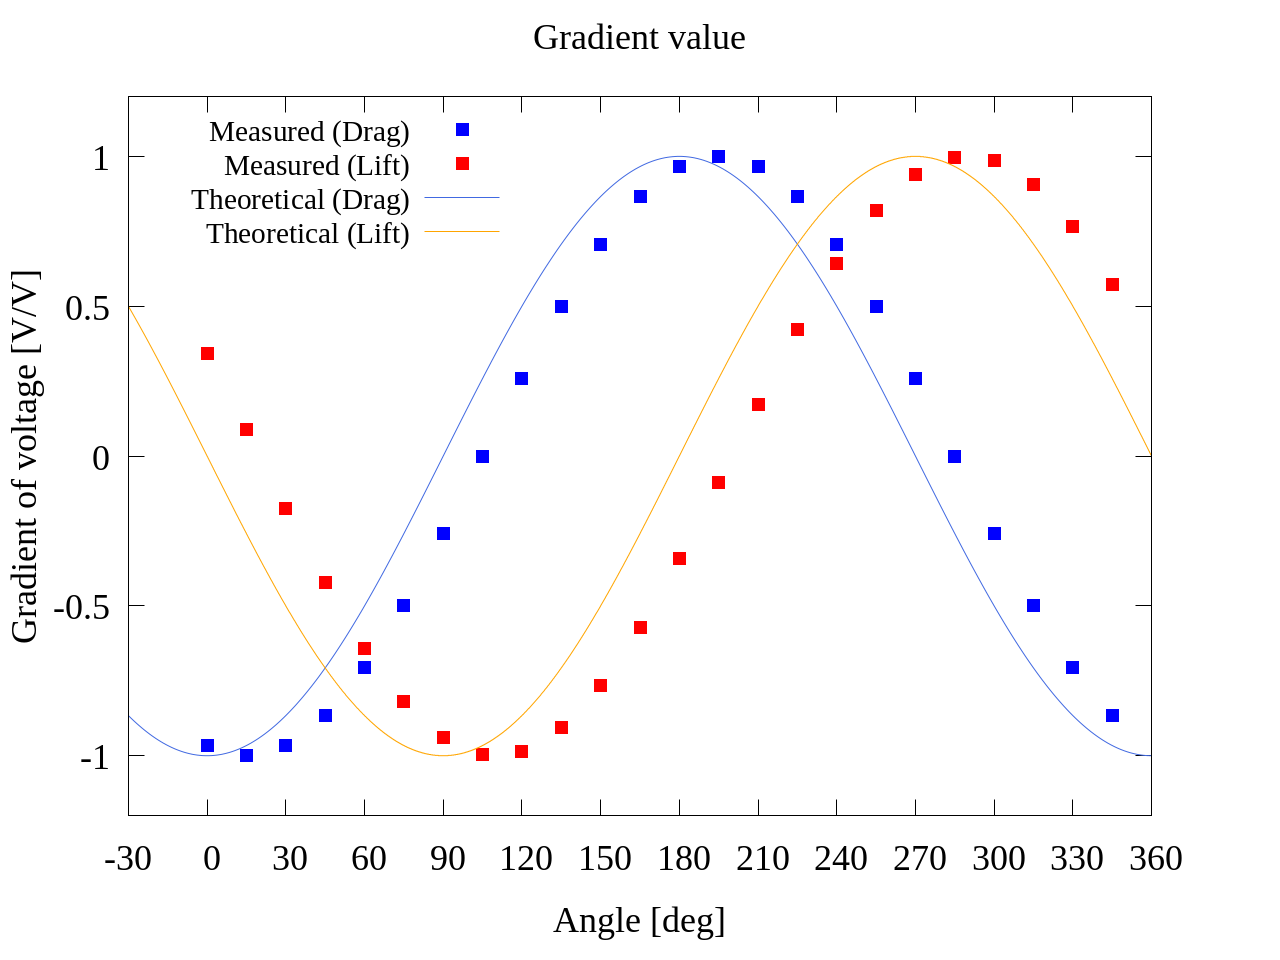
\includegraphics[width=95mm]{../../02_workspace/result/rotation_tx=15.0_ty=20.0/plot/20/20_adjust-value.png}
    \caption{Simulated gradient [Case 1]}
  \end{center}
\end{figure}

\newpage

Fig.10をみると,理論値の曲線とプロットされたテストデータに位相差があることがわかる.
このとき,テストデータに離散フーリ変換を適用すると波数1の成分についてTable 2のような値を得ることができる.
また,そのときのスペクトルをFig.11 に示す.

\begin{table}[htbp]
  \begin{center}
    \caption{DFT spectrum [Case 1]}
    \begin{tabular}{|p{30mm}|p{20mm}|p{20mm}|}
      \hline
      \multicolumn{1}{|c|}{}     & \multicolumn{1}{|c|}{Re}      & \multicolumn{1}{|c|}{Im}     \\ \hline
      \multicolumn{1}{|c|}{Drag} & \multicolumn{1}{|c|}{-11.591} & \multicolumn{1}{|c|}{3.106}  \\ \hline
      \multicolumn{1}{|c|}{Lift} & \multicolumn{1}{|c|}{4.104}   & \multicolumn{1}{|c|}{11.276} \\ \hline
    \end{tabular}
  \end{center}
\end{table}

\begin{figure}[htbp]
  \begin{minipage}[b]{0.45\linewidth}
    \centering
    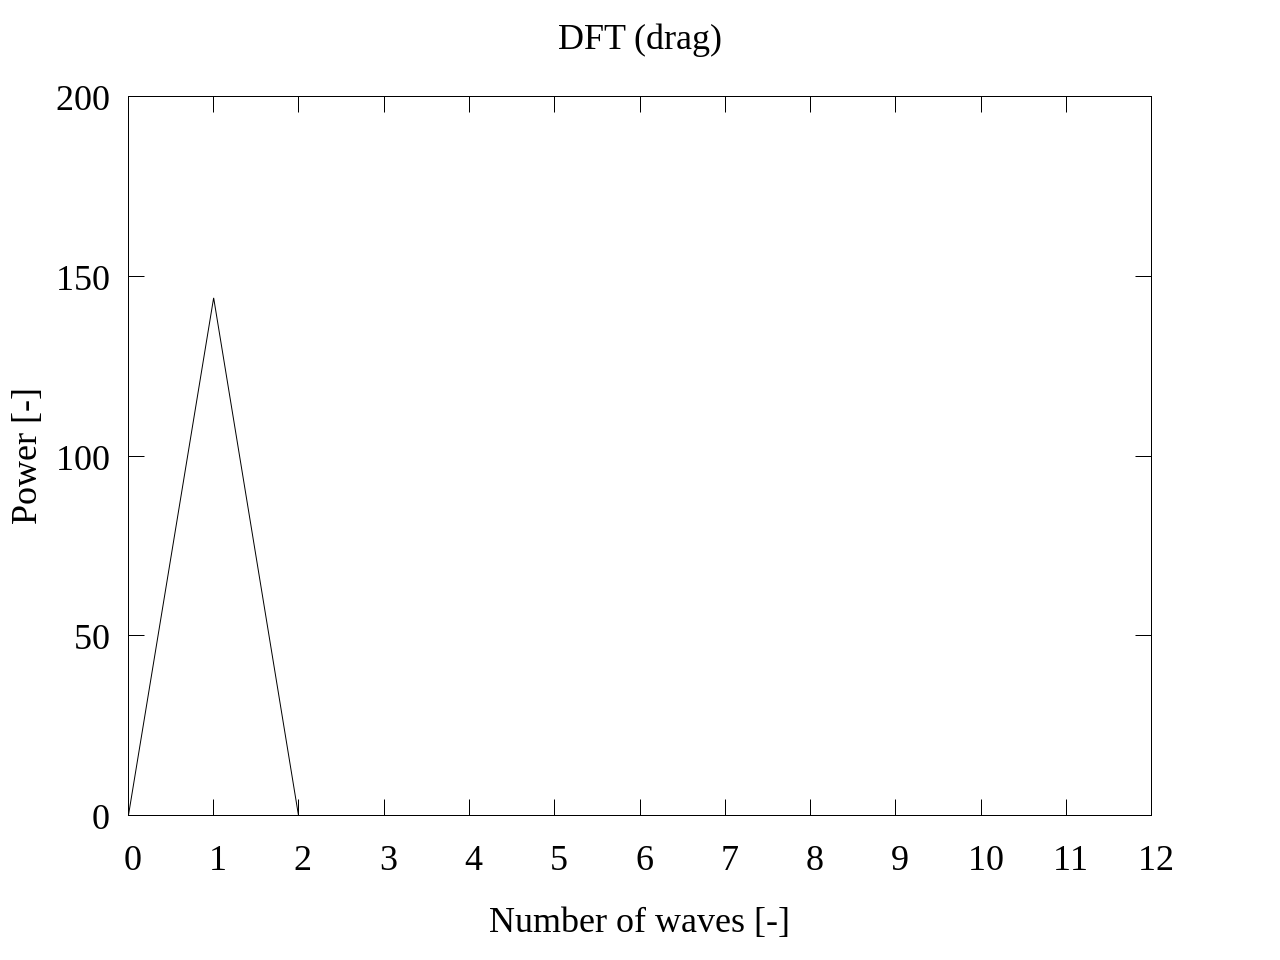
\includegraphics[width=65mm]{../../02_workspace/result/rotation_tx=15.0_ty=20.0/plot/07/07-3_dft-drag.png}
    \subcaption{Drag}
  \end{minipage}
  \begin{minipage}[b]{0.45\linewidth}
    \centering
    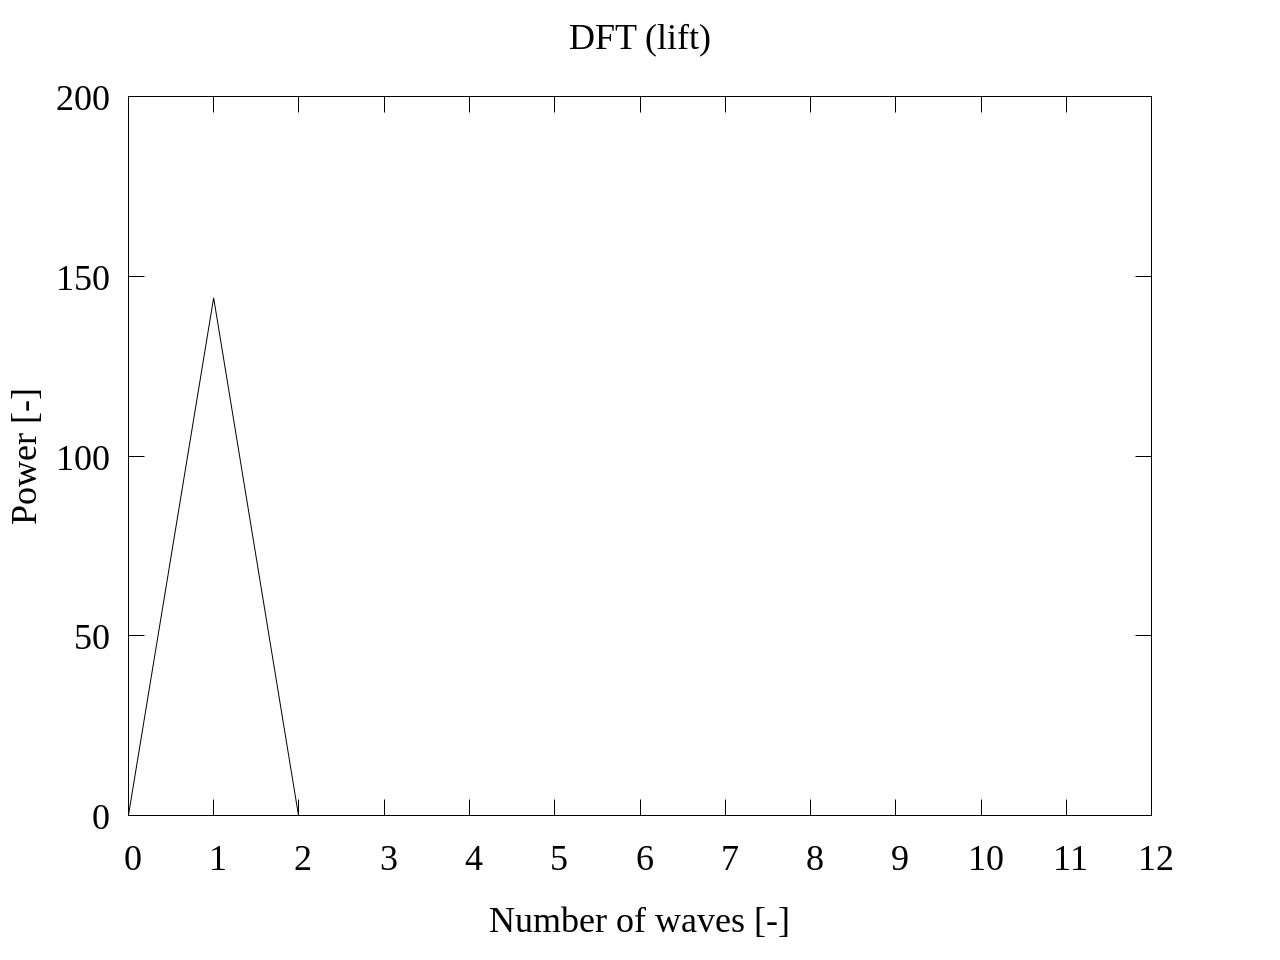
\includegraphics[width=65mm]{../../02_workspace/result/rotation_tx=15.0_ty=20.0/plot/07/07-4_dft-lift.png}
    \subcaption{Lift}
  \end{minipage}
  \caption{DFT spectrum [Case 1]}
\end{figure}

Fig.11 より,波数1についてピークがあることがわかり,データの特徴を正しく捉えられているといえる.
ここで,Table 2について,式(5)より位相角$\phi_{1\;\mathrm{test}}$,$\phi_{2\;\mathrm{test}}$をそれぞれ算出する.

\begin{align}
  \phi_{1\;,\mathrm{test}} & = \arctan \left(\frac{3.106}{-11.591} \right) \cdot \frac{180}{\pi} = 165.000 \;\mathrm{[deg]} \\
  \notag                                                                                                                    \\
  \phi_{2\;,\mathrm{test}} & = \arctan \left(\frac{11.276}{4.101}\right) \cdot \frac{180}{\pi} = 70.000 \;\mathrm{[deg]}
\end{align}
\vskip \baselineskip

式(6),式(7)より算出した位相角を用いて位相差$\theta_{x \;\mathrm{test}}$,$\theta_{y \;\mathrm{test}}$を求める.

\begin{align}
  \theta_{x\;,\mathrm{test}} & = \pi \cdot \frac{180}{\pi} - 165 = 15\;\mathrm{[deg]}          \\
  \notag                                                                                       \\
  \theta_{y\;,\mathrm{test}} & = \frac{\pi}{2} \cdot \frac{180}{\pi} - 70 = 20\;\mathrm{[deg]}
\end{align}

\newpage
また,位相差$\theta_{x \;\mathrm{test}}$,$\theta_{y \;\mathrm{test}}$より,
ひずみセンサの取付角$\phi_{s\;\mathrm{test}}$が式(8)よりわかる.

\begin{align}
  \phi_{s\;\mathrm{test}} = \left|15 - 20\right| = 5 \;[\mathrm{deg} ]
\end{align}

次に,位相差位相差$\theta_{x,\;\mathrm{test}}$,$\theta_{y,\;\mathrm{test}}$,
テストデータから得られる$v_{x',\;\mathrm{test}}$,$v_{xy,\;\mathrm{test}}$より,
水槽座標系における出力電圧勾配$v_x$,$v_y$を
式(1),式(2)を用いて算出する.それぞれの角度についての算出結果をTable 3,Fig.12 に示す.

\begin{table}[htbp]
  \begin{center}
    \caption{Correction test [Case 1]}
    \begin{tabular}{|p{20mm}|p{20mm}|p{20mm}|p{20mm}|p{20mm}|}
      \hline
      \multicolumn{1}{|c|}{\textgt{$\varphi$ [deg]}} & \multicolumn{1}{|c|}{\textgt{$v_{x'\;\mathrm{test}}$ [V/V]}} & \multicolumn{1}{|c|}{\textgt{$v_{xy\;\mathrm{test}}$ [V/V]}} & \multicolumn{1}{|c|}{\textgt{$v_x$ [V/V]}} & \multicolumn{1}{|c|}{\textgt{$v_y$ [V/V]}} \\ \hline
      \multicolumn{1}{|c|}{0}                        & \multicolumn{1}{|r|}{-0.966}                                 & \multicolumn{1}{|r|}{0.342}                                  & \multicolumn{1}{|r|}{-1.000}               & \multicolumn{1}{|r|}{0.000}                \\ \hline
      \multicolumn{1}{|c|}{15}                       & \multicolumn{1}{|r|}{-1.000}                                 & \multicolumn{1}{|r|}{0.087}                                  & \multicolumn{1}{|r|}{-0.966}               & \multicolumn{1}{|r|}{-0.259}               \\ \hline
      \multicolumn{1}{|c|}{30}                       & \multicolumn{1}{|r|}{-0.966}                                 & \multicolumn{1}{|r|}{-0.174}                                 & \multicolumn{1}{|r|}{-0.866}               & \multicolumn{1}{|r|}{-0.500}               \\ \hline
      \multicolumn{1}{|c|}{45}                       & \multicolumn{1}{|r|}{-0.866}                                 & \multicolumn{1}{|r|}{-0.423}                                 & \multicolumn{1}{|r|}{-0.707}               & \multicolumn{1}{|r|}{-0.707}               \\ \hline
      \multicolumn{1}{|c|}{60}                       & \multicolumn{1}{|r|}{-0.707}                                 & \multicolumn{1}{|r|}{-0.643}                                 & \multicolumn{1}{|r|}{-0.500}               & \multicolumn{1}{|r|}{-0.866}               \\ \hline
      \multicolumn{1}{|c|}{75}                       & \multicolumn{1}{|r|}{-0.500}                                 & \multicolumn{1}{|r|}{-0.819}                                 & \multicolumn{1}{|r|}{-0.259}               & \multicolumn{1}{|r|}{-0.966}               \\ \hline
      \multicolumn{1}{|c|}{90}                       & \multicolumn{1}{|r|}{-0.259}                                 & \multicolumn{1}{|r|}{-0.940}                                 & \multicolumn{1}{|r|}{0.000}                & \multicolumn{1}{|r|}{-1.000}               \\ \hline
      \multicolumn{1}{|c|}{105}                      & \multicolumn{1}{|r|}{0.000}                                  & \multicolumn{1}{|r|}{-0.996}                                 & \multicolumn{1}{|r|}{0.259}                & \multicolumn{1}{|r|}{-0.966}               \\ \hline
      \multicolumn{1}{|c|}{120}                      & \multicolumn{1}{|r|}{0.259}                                  & \multicolumn{1}{|r|}{-0.985}                                 & \multicolumn{1}{|r|}{0.500}                & \multicolumn{1}{|r|}{-0.866}               \\ \hline
      \multicolumn{1}{|c|}{135}                      & \multicolumn{1}{|r|}{0.500}                                  & \multicolumn{1}{|r|}{-0.906}                                 & \multicolumn{1}{|r|}{0.707}                & \multicolumn{1}{|r|}{-0.707}               \\ \hline
      \multicolumn{1}{|c|}{150}                      & \multicolumn{1}{|r|}{0.707}                                  & \multicolumn{1}{|r|}{-0.766}                                 & \multicolumn{1}{|r|}{0.866}                & \multicolumn{1}{|r|}{-0.500}               \\ \hline
      \multicolumn{1}{|c|}{165}                      & \multicolumn{1}{|r|}{0.866}                                  & \multicolumn{1}{|r|}{-0.574}                                 & \multicolumn{1}{|r|}{0.966}                & \multicolumn{1}{|r|}{-0.259}               \\ \hline
      \multicolumn{1}{|c|}{180}                      & \multicolumn{1}{|r|}{0.966}                                  & \multicolumn{1}{|r|}{-0.342}                                 & \multicolumn{1}{|r|}{1.000}                & \multicolumn{1}{|r|}{-0.000}               \\ \hline
      \multicolumn{1}{|c|}{195}                      & \multicolumn{1}{|r|}{1.000}                                  & \multicolumn{1}{|r|}{-0.087}                                 & \multicolumn{1}{|r|}{0.966}                & \multicolumn{1}{|r|}{0.259}                \\ \hline
      \multicolumn{1}{|c|}{210}                      & \multicolumn{1}{|r|}{0.966}                                  & \multicolumn{1}{|r|}{0.174}                                  & \multicolumn{1}{|r|}{0.866}                & \multicolumn{1}{|r|}{0.500}                \\ \hline
      \multicolumn{1}{|c|}{225}                      & \multicolumn{1}{|r|}{0.866}                                  & \multicolumn{1}{|r|}{0.423}                                  & \multicolumn{1}{|r|}{0.707}                & \multicolumn{1}{|r|}{0.707}                \\ \hline
      \multicolumn{1}{|c|}{240}                      & \multicolumn{1}{|r|}{0.707}                                  & \multicolumn{1}{|r|}{0.643}                                  & \multicolumn{1}{|r|}{0.500}                & \multicolumn{1}{|r|}{0.866}                \\ \hline
      \multicolumn{1}{|c|}{255}                      & \multicolumn{1}{|r|}{0.500}                                  & \multicolumn{1}{|r|}{0.819}                                  & \multicolumn{1}{|r|}{0.259}                & \multicolumn{1}{|r|}{0.966}                \\ \hline
      \multicolumn{1}{|c|}{270}                      & \multicolumn{1}{|r|}{0.259}                                  & \multicolumn{1}{|r|}{0.940}                                  & \multicolumn{1}{|r|}{-0.000}               & \multicolumn{1}{|r|}{1.000}                \\ \hline
      \multicolumn{1}{|c|}{285}                      & \multicolumn{1}{|r|}{-0.000}                                 & \multicolumn{1}{|r|}{0.996}                                  & \multicolumn{1}{|r|}{-0.259}               & \multicolumn{1}{|r|}{0.966}                \\ \hline
      \multicolumn{1}{|c|}{300}                      & \multicolumn{1}{|r|}{-0.259}                                 & \multicolumn{1}{|r|}{0.985}                                  & \multicolumn{1}{|r|}{-0.500}               & \multicolumn{1}{|r|}{0.866}                \\ \hline
      \multicolumn{1}{|c|}{315}                      & \multicolumn{1}{|r|}{-0.500}                                 & \multicolumn{1}{|r|}{0.906}                                  & \multicolumn{1}{|r|}{-0.707}               & \multicolumn{1}{|r|}{0.707}                \\ \hline
      \multicolumn{1}{|c|}{330}                      & \multicolumn{1}{|r|}{-0.707}                                 & \multicolumn{1}{|r|}{0.766}                                  & \multicolumn{1}{|r|}{-0.866}               & \multicolumn{1}{|r|}{0.500}                \\ \hline
      \multicolumn{1}{|c|}{345}                      & \multicolumn{1}{|r|}{-0.866}                                 & \multicolumn{1}{|r|}{0.574}                                  & \multicolumn{1}{|r|}{-0.966}               & \multicolumn{1}{|r|}{0.259}                \\ \hline
    \end{tabular}
  \end{center}
\end{table}

\begin{figure}[htbp]
  \begin{center}
    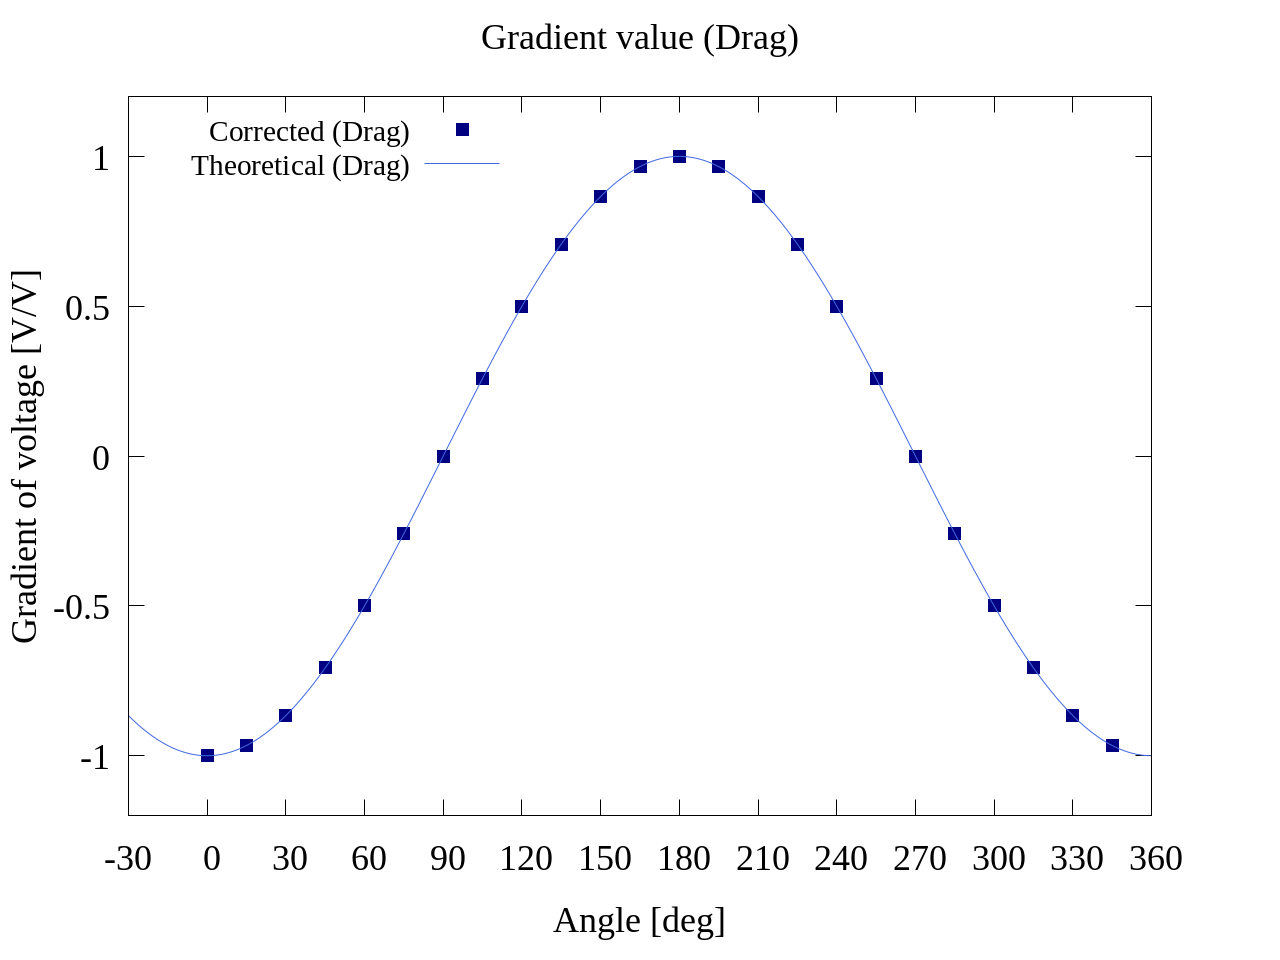
\includegraphics[width=95mm]{../../02_workspace/result/rotation_tx=15.0_ty=20.0/plot/21/21-4_corrected_angle_drag.png}
    \subcaption{Drag}
    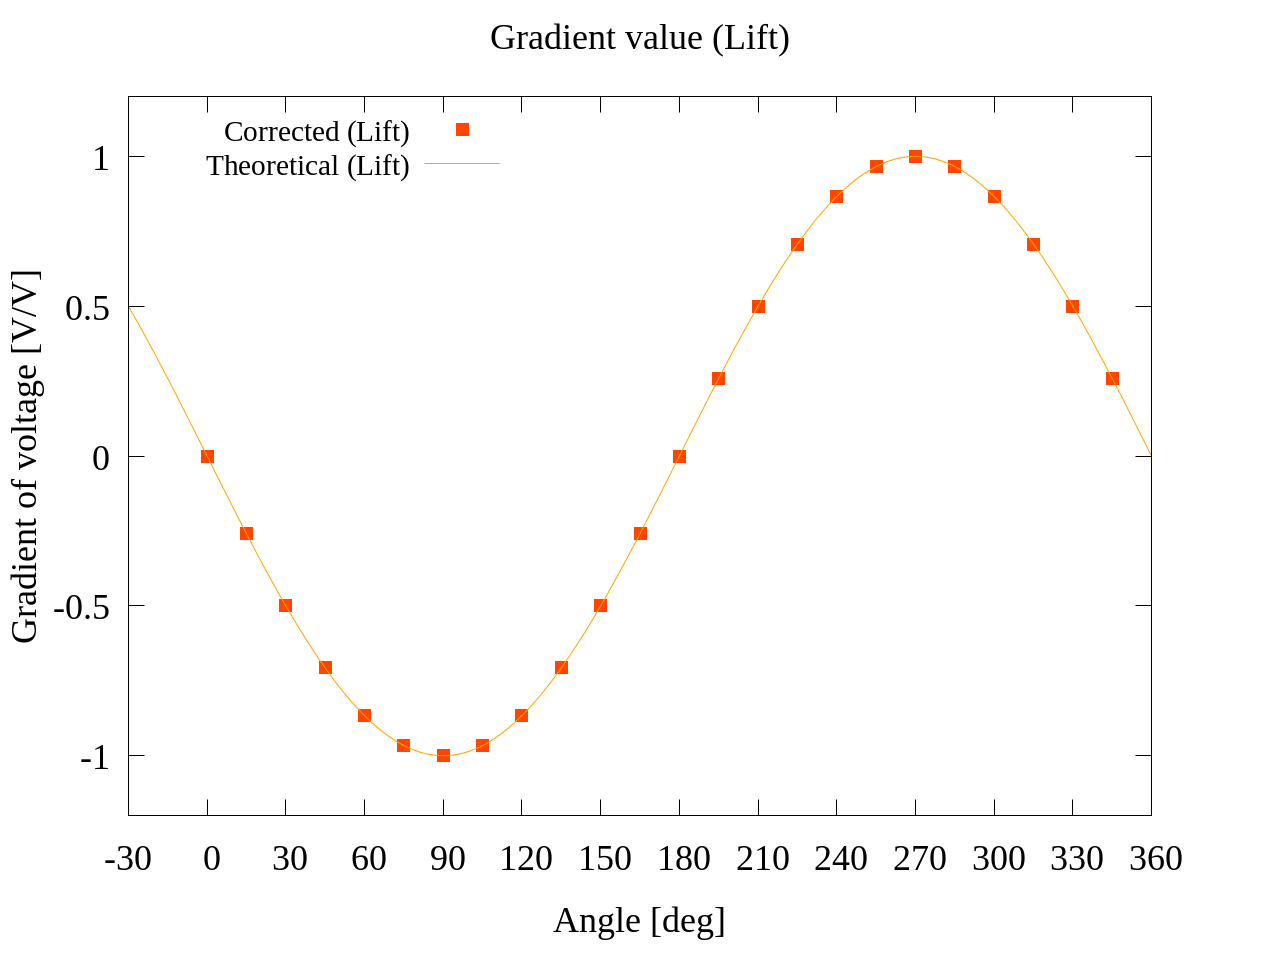
\includegraphics[width=95mm]{../../02_workspace/result/rotation_tx=15.0_ty=20.0/plot/21/21-4_corrected_angle_lift.png}
    \subcaption{Lift}
  \end{center}
  \caption{Corrected gradient [Case 1]}
\end{figure}

Fig.をみると算出された補正値すなわち水槽座標系における出力電圧勾配は,
理論曲線状に位置していることが確認でき,正しく算出されていることがわかる.

\newpage
また,Fig.13,Fig.14に,Case2 および Case3 におけるテストデータとその補正結果について示す.

\subsubsection{テストデータ : Case 2 ($\theta_{x \mathrm{test}} = -15 \; \mathrm{[deg]}$, $\theta_{y \mathrm{test}} = -20 \; \mathrm{[deg]}$)}


\begin{figure}[htbp]
  \begin{minipage}[b]{0.45\linewidth}
    \centering
    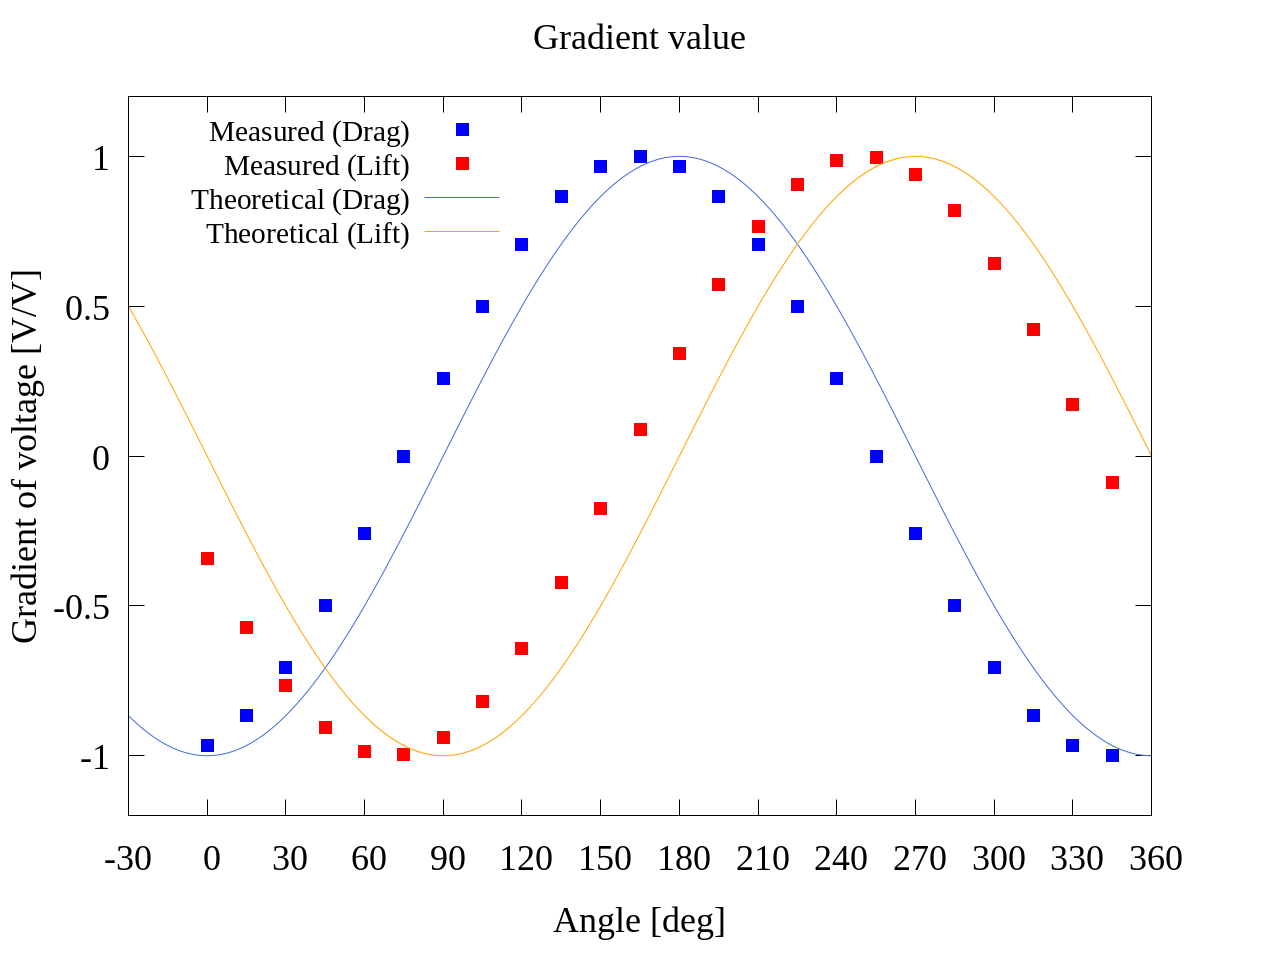
\includegraphics[width=65mm]{../../02_workspace/result/rotation_tx=-15.0_ty=-20.0/plot/20/20_adjust-value.png}
    \subcaption{Simulated gradient}
  \end{minipage}
  \begin{minipage}[b]{0.45\linewidth}
    \centering
    \includegraphics[width=65mm]{../../02_workspace/result/rotation_tx=-15.0_ty=-20.0/plot/21/21-4_summary.png}
    \subcaption{Corrected gradient}
  \end{minipage}
  \caption{Test data [Case 2]}
\end{figure}

\subsubsection{テストデータ : Case 3 ($\theta_{x \mathrm{test}} = 90 \; \mathrm{[deg]}$, $\theta_{y \mathrm{test}} = -90 \; \mathrm{[deg]}$)}

\begin{figure}[htbp]
  \begin{minipage}[b]{0.45\linewidth}
    \centering
    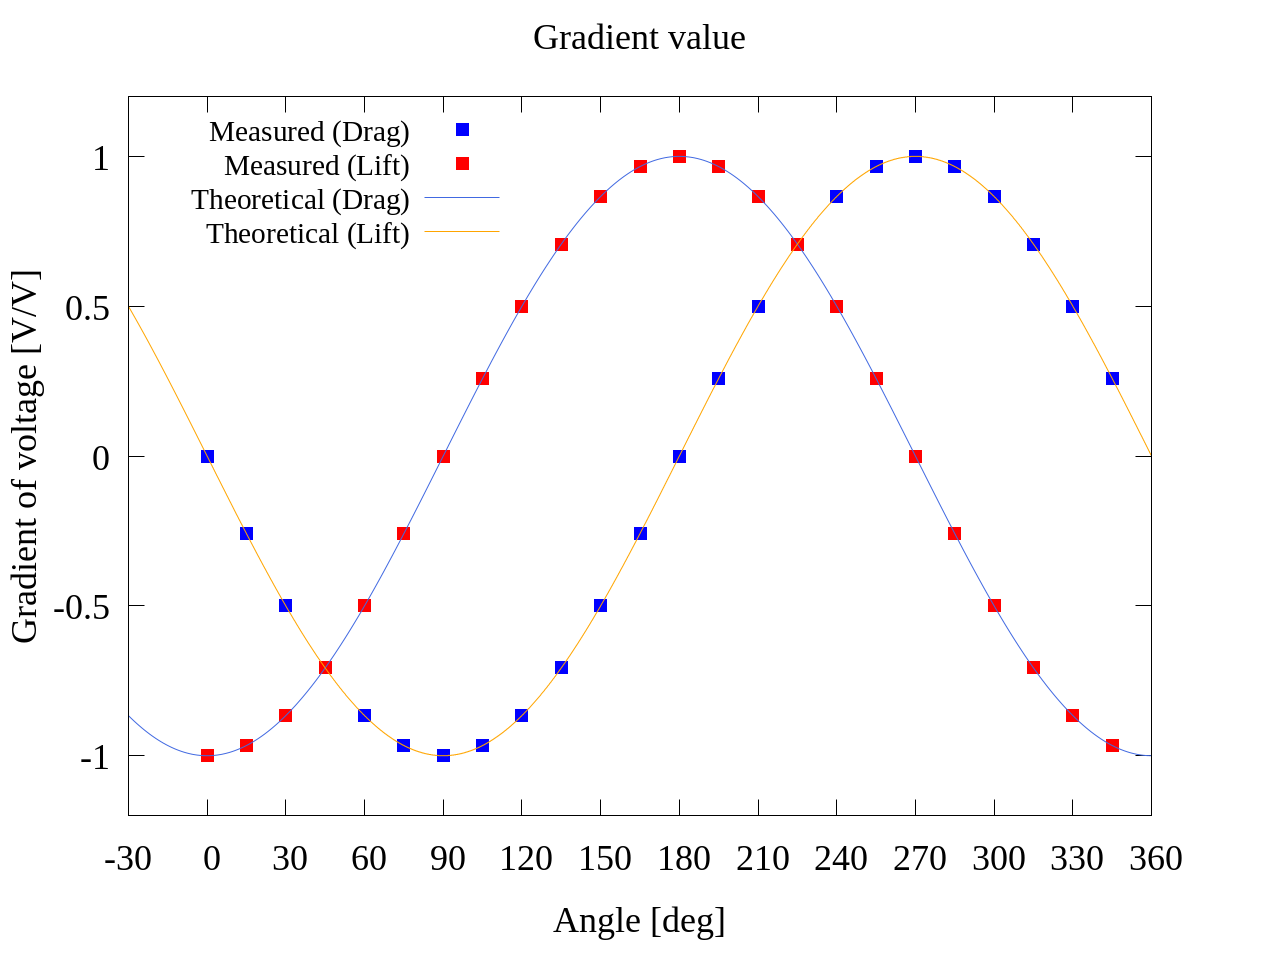
\includegraphics[width=65mm]{../../02_workspace/result/rotation_tx=90.0_ty=-90.0/plot/20/20_adjust-value.png}
    \subcaption{Simulated gradient}
  \end{minipage}
  \begin{minipage}[b]{0.45\linewidth}
    \centering
    \includegraphics[width=65mm]{../../02_workspace/result/rotation_tx=90.0_ty=-90.0/plot/21/21-4_summary.png}
    \subcaption{Corrected gradient}
  \end{minipage}
  \caption{Test data [Case 3]}
\end{figure}

ここで,Fig.13,Fig.14をみると回転角度が負の値の場合,その値が非常に大きい場合であっても
問題なく補正処理が可能であることがわかる.
したがって,補正理論[1]はテストデータについて正しく機能しており,
水槽座標系と座標系Aの回転角および作用力測定装置のひずみセンサの取付角,
水槽座標系における出力電圧勾配を調べることができる.

\newpage
\subsection{補正理論[2] : 座標系のオフセットにおける補正理論}

次に,水槽座標系と座標系Bのオフセットの補正理論を説明する.
ここでは,Fig.15に示すように回転角はなく,
水槽座標系の中心oと座標系Bの中心o''はオフセット$\Delta x$,$\Delta y$を持つ.
ここで,作用力$F$を与えるとき,その作用線はオフセット$\Delta x$,$\Delta y$によって
水槽座標系の中心oを通ることはなく,座標系Bの中心o''を通る.
このとき,作用点$f$と点o''を通る直線(青点線)と$x''$軸の角度を$\theta$,
作用点$f$と点oを通る直線(赤点線)と$x$軸の角度を$\varphi$とする.
また,作用点$f$と点o''を通る直線(青点線)と作用点$f$と点oを通る直線(赤点線)の角度を$\alpha$とする.
角度$\theta$は校正実験時に記録される角度となる.

\begin{figure}[htbp]
  \begin{center}
    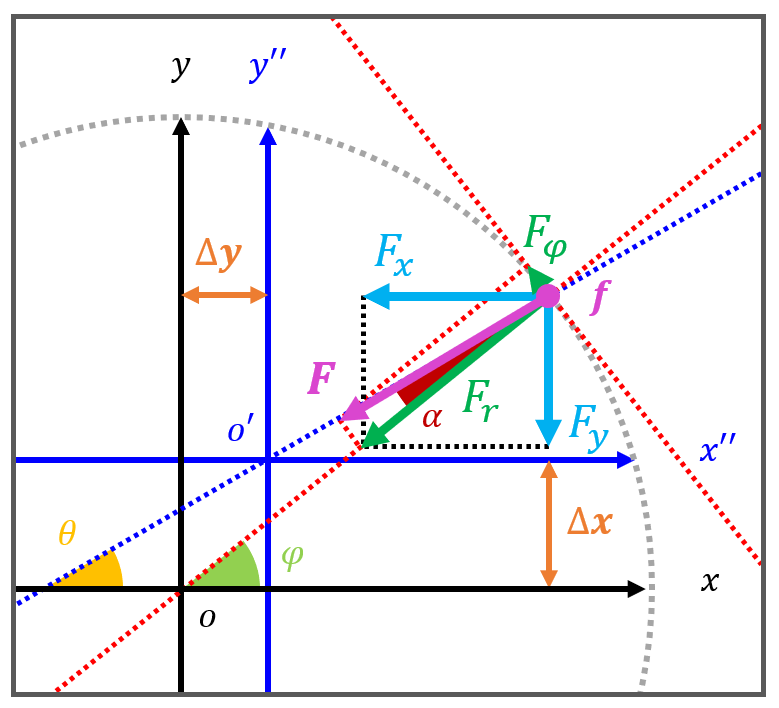
\includegraphics[width=65mm]{images/34-1.png}
    \caption{Relationship between ($x-y$) and ($x''-y''$)}
  \end{center}
\end{figure}

\subsubsection{角度$\alpha$の算出}
供試体の半径を$r$とするとき,水槽座標系について
作用点$f$の$(x,y)$座標は角度$\varphi$を用いて以下のように表すことができる.

\begin{align}
  x & = r \cos \varphi \\
  y & = r \sin \varphi
\end{align}

\newpage

また,座標系Bについて考える,
このとき作用点$f$の$(x'',y'')$の座標はオフセット$\Delta x$,$\Delta y$を用いて
以下のように表される.

\begin{align}
  x'' & = r \cos \varphi -\Delta x \\
  y'' & = r \sin \varphi -\Delta y
\end{align}
\vskip \baselineskip

以上より,角度$\theta$を用いて角度$\varphi$を求めることができる.

\begin{align}
  \tan \theta & = \frac{y''}{x''} = \frac{ r \sin \varphi - \Delta y}{ r \cos \varphi - \Delta x}      \\
  \notag                                                                                               \\
  \varphi     & = \theta - \sin^{-1}\left(\frac{\Delta x \sin \theta - \Delta y \cos \theta}{r}\right)
\end{align}
\vskip \baselineskip

したがって,角度$\alpha$を以下のように求めることができる.

\begin{align}
  \alpha = \theta - \varphi = \sin^{-1} \left( \frac{\Delta x \sin \theta - \Delta y \cos \theta}{r} \right)
\end{align}
\vskip \baselineskip

\subsubsection{作用力$F$の分解}

供試体に加わる作用力$F$は供試体表面の接線方向の力$F_\varphi$,
またその法線方向の力$F_r$に分けて考えることができる.
ロードセルから与える作用力の角度$\theta$,算出した$\varphi$を用いると,それぞれ以下のように求められる.

\begin{align}
  F_{\varphi} & = F \sin \alpha = F \sin \left(\theta - \varphi\right) \\
  F_{r}       & = F \cos \alpha = F \cos \left(\theta - \varphi\right)
\end{align}
\vskip \baselineskip

供試体への作用力について抗力方向を$F_{x}$,揚力方向を$F_{y}$とすると
角度$\varphi$を用いて以下のように求められる.

\begin{align}
  F_{x} & = - F_r \cos \varphi \\
  F_{y} & = - F_r \sin \varphi
\end{align}

\newpage
また,接線方向成分$F_\varphi$について,供試体に対してトルク$T$として作用することとなる.
ここで,このトルク$T$について,
作用力測定装置に対する影響は十分に小さいと考えられることから無視する.\\

\begin{align}
  T & = F_\varphi \cdot r = F \sin \alpha \cdot r
\end{align}
\vskip \baselineskip

\subsubsection{出力電圧勾配の座標系変換 (2)}

水槽座標系に対して,オフセットを持つ座標系Bを基準に
ロードセルから与えられる作用力$F$はすべて作用力測定装置の中心に伝わることはなく,
接線方向の力$F_r$,その法線方向の力$F_\theta$に分解される.
すなわち,測定時にはロードセルから作用力$F$を与えた際の出力電圧,
ひずみセンサから作用力$F_r$を与えた際の出力電圧を得ているということになる.
したがって,ひずみセンサの出力電圧の傾きを一様に評価することは不可能であり,
実際の作用力$F_r$の角度$\alpha$を算出し補正を加える必要がある.

ここで,ひずみセンサの出力電圧$V_{x''2}$,$V_{y''2}$は
それぞれ$F_r / F$倍されていると考えられることから,
水槽座標系における出力電圧勾配$v_{x}$,$v_{y}$と
座標系Bにおける出力電圧勾配$v_{x''2}$,$v_{y''2}$は
角度$\alpha$を用いて以下のような関係が成立する.

\begin{align}
  v_{x} & = \frac{F}{F_r} v_{x''2} = \frac{1}{\cos \alpha} v_{x''2} \\
  \notag                                                            \\
  v_{y} & = \frac{F}{F_r} v_{y''2} = \frac{1}{\cos \alpha} v_{y''2}
\end{align}

\subsubsection{補正理論[2]のテストデータへの適用}

以上の補正理論より,オフセットを考慮したテストデータを構成する.
任意のオフセット$\Delta x_\mathrm{test}$,$\Delta y_\mathrm{test}$を与えて
座標系Bの出力電圧勾配について,$x''$軸方向を$v_{x''\;\mathrm{test}}$,
$y''$軸方向を$v_{y''\;\mathrm{test}}$とするとき,以下のように表される.
また,今回はTable 4のようなパラメータを用いてテストデータを構成した.

\begin{align}
  \theta                  & = \frac{\pi}{180} \; i \;\left(i = 0, 1, 2, 3, \cdots\right)                                                       \\
  \alpha                  & = \sin^{-1} \left( \frac{\Delta x_\mathrm{test} \sin \theta - \Delta y_\mathrm{test} \cos \theta}{r} \right)       \\
  \varphi                 & = \theta - \sin^{-1}\left(\frac{\Delta x_\mathrm{test} \sin \theta - \Delta y_\mathrm{test} \cos \theta}{r}\right) \\
  v_{x'' \;\mathrm{test}} & = - \cos \alpha \cos \varphi                                                                                       \\
  v_{y'' \;\mathrm{test}} & = - \cos \alpha \sin \varphi
\end{align}

\begin{table}[htbp]
  \begin{center}
    \caption{Test data conditions [2]}
    \begin{tabular}{|p{30mm}|p{20mm}|p{20mm}|}
      \hline
      \multicolumn{1}{|c|}{}       & \multicolumn{1}{|c|}{$\Delta x_\mathrm{test}$ [mm]} & \multicolumn{1}{|c|}{$\Delta y_\mathrm{test}$ [mm]} \\ \hline
      \multicolumn{1}{|c|}{Case 4} & \multicolumn{1}{|c|}{5.0}                           & \multicolumn{1}{|c|}{0.0}                           \\ \hline
      \multicolumn{1}{|c|}{Case 5} & \multicolumn{1}{|c|}{5.0}                           & \multicolumn{1}{|c|}{-5.0}                          \\ \hline
      \multicolumn{1}{|c|}{Case 6} & \multicolumn{1}{|c|}{10.0}                          & \multicolumn{1}{|c|}{-5.0}                          \\ \hline
    \end{tabular}
  \end{center}
\end{table}

ここで,Case 4 に対する座標系の回転おける補正理論の適用過程について説明する.
はじめに,構成したテストデータを以下に示す.

\begin{figure}[htbp]
  \begin{center}
    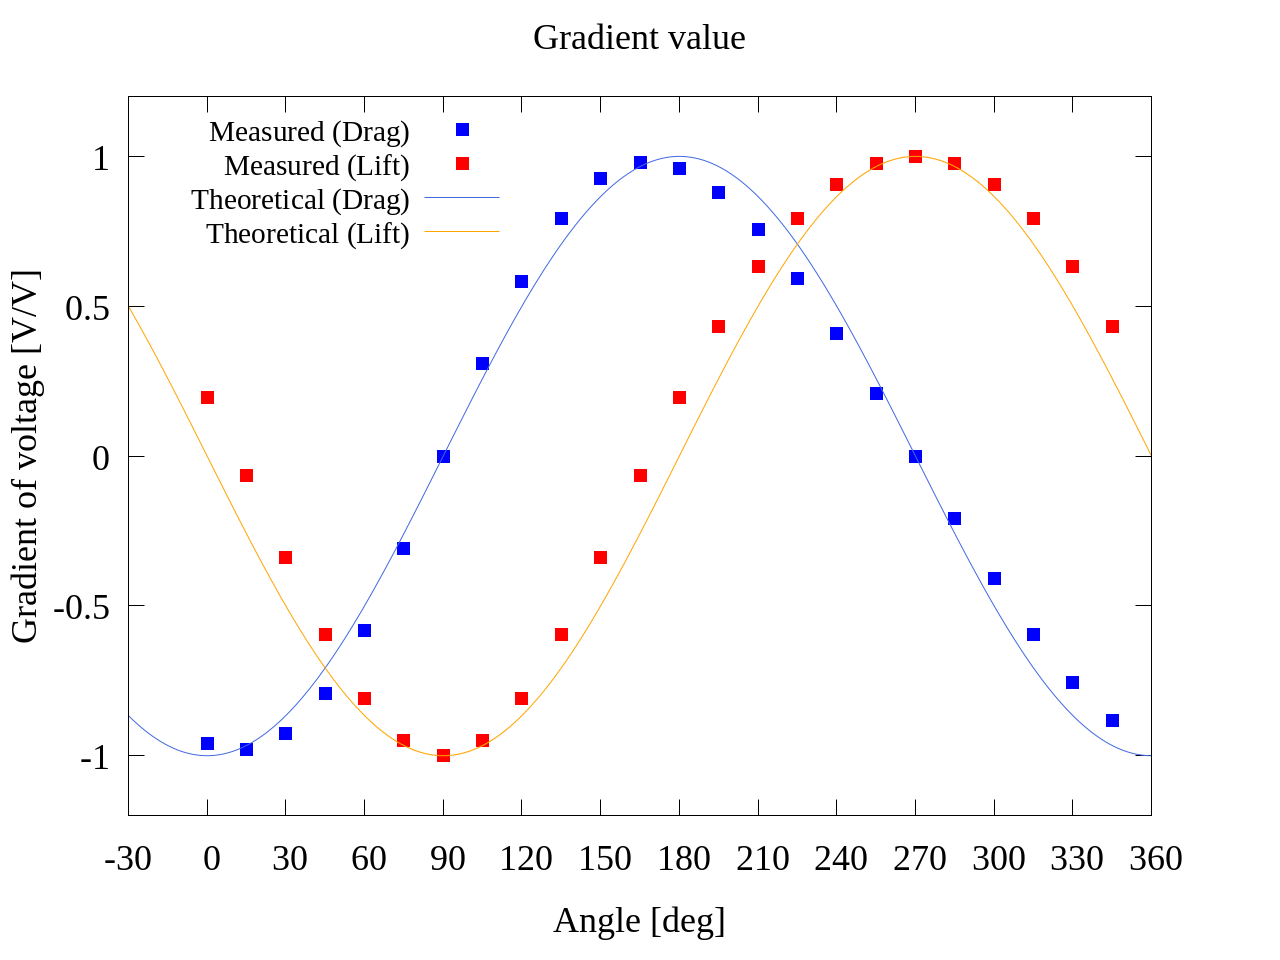
\includegraphics[width=95mm]{../../02_workspace/result/offset_dx=5.0_dy=0.0/plot/20/20_adjust-value.png}
    \caption{Simulated gradient [Case 4]}
  \end{center}
\end{figure}
\vskip \baselineskip

Fig.16をみると,プロットされたテストデータは理論値の曲線とは異なる値を示している.
また,波形は少し不規則な形状となっていることがわかる.

\newpage

ここで,$\theta$,$\Delta x_\mathrm{test}$,$\Delta y_\mathrm{test}$は既知の変数であるため
式(31),式(32)より,$\alpha$および$\varphi$を求めることができる.
したがって,式(38),式(39)を適用した結果を5に示す.
ここで,$\varphi$は水槽座標系において供試体へ作用力が加えられている角度を示していることになる.

\begin{table}[htbp]
  \begin{center}
    \caption{Correction test [Case 4]}
    \begin{tabular}{|p{15 mm}|p{15 mm}|p{15 mm}|p{15 mm}|p{15 mm}|p{15 mm}|}
      \hline
      \multicolumn{1}{|c|}{\textgt{Angle [deg]}} & \multicolumn{1}{|c|}{\textgt{$v_{x''\;\mathrm{test}}$ [V/V]}} & \multicolumn{1}{|c|}{\textgt{$v_{y''\;\mathrm{test}}$ [V/V]}} & \multicolumn{1}{|c|}{\textgt{$v_x$ [V/V]}} & \multicolumn{1}{|c|}{\textgt{$v_y$ [V/V]}} & \multicolumn{1}{|c|}{\textgt{$\varphi$ [deg]}} \\ \hline
      \multicolumn{1}{|c|}{0}                    & \multicolumn{1}{|r|}{-0.960}                                  & \multicolumn{1}{|r|}{0.196}                                   & \multicolumn{1}{|r|}{-0.980}               & \multicolumn{1}{|r|}{0.200}                & \multicolumn{1}{|r|}{-11.5}                    \\ \hline
      \multicolumn{1}{|c|}{15}                   & \multicolumn{1}{|r|}{-0.979}                                  & \multicolumn{1}{|r|}{-0.066}                                  & \multicolumn{1}{|r|}{-0.998}               & \multicolumn{1}{|r|}{-0.067}               & \multicolumn{1}{|r|}{3.9}                      \\ \hline
      \multicolumn{1}{|c|}{30}                   & \multicolumn{1}{|r|}{-0.925}                                  & \multicolumn{1}{|r|}{-0.337}                                  & \multicolumn{1}{|r|}{-0.940}               & \multicolumn{1}{|r|}{-0.342}               & \multicolumn{1}{|r|}{20.0}                     \\ \hline
      \multicolumn{1}{|c|}{45}                   & \multicolumn{1}{|r|}{-0.792}                                  & \multicolumn{1}{|r|}{-0.594}                                  & \multicolumn{1}{|r|}{-0.800}               & \multicolumn{1}{|r|}{-0.600}               & \multicolumn{1}{|r|}{36.9}                     \\ \hline
      \multicolumn{1}{|c|}{60}                   & \multicolumn{1}{|r|}{-0.581}                                  & \multicolumn{1}{|r|}{-0.808}                                  & \multicolumn{1}{|r|}{-0.584}               & \multicolumn{1}{|r|}{-0.812}               & \multicolumn{1}{|r|}{54.3}                     \\ \hline
      \multicolumn{1}{|c|}{75}                   & \multicolumn{1}{|r|}{-0.308}                                  & \multicolumn{1}{|r|}{-0.950}                                  & \multicolumn{1}{|r|}{-0.308}               & \multicolumn{1}{|r|}{-0.951}               & \multicolumn{1}{|r|}{72.0}                     \\ \hline
      \multicolumn{1}{|c|}{90}                   & \multicolumn{1}{|r|}{-0.000}                                  & \multicolumn{1}{|r|}{-1.000}                                  & \multicolumn{1}{|r|}{-0.000}               & \multicolumn{1}{|r|}{-1.000}               & \multicolumn{1}{|r|}{90.0}                     \\ \hline
      \multicolumn{1}{|c|}{105}                  & \multicolumn{1}{|r|}{0.308}                                   & \multicolumn{1}{|r|}{-0.950}                                  & \multicolumn{1}{|r|}{0.308}                & \multicolumn{1}{|r|}{-0.951}               & \multicolumn{1}{|r|}{108.0}                    \\ \hline
      \multicolumn{1}{|c|}{120}                  & \multicolumn{1}{|r|}{0.581}                                   & \multicolumn{1}{|r|}{-0.808}                                  & \multicolumn{1}{|r|}{0.584}                & \multicolumn{1}{|r|}{-0.812}               & \multicolumn{1}{|r|}{125.7}                    \\ \hline
      \multicolumn{1}{|c|}{135}                  & \multicolumn{1}{|r|}{0.792}                                   & \multicolumn{1}{|r|}{-0.594}                                  & \multicolumn{1}{|r|}{0.800}                & \multicolumn{1}{|r|}{-0.600}               & \multicolumn{1}{|r|}{143.1}                    \\ \hline
      \multicolumn{1}{|c|}{150}                  & \multicolumn{1}{|r|}{0.925}                                   & \multicolumn{1}{|r|}{-0.337}                                  & \multicolumn{1}{|r|}{0.940}                & \multicolumn{1}{|r|}{-0.342}               & \multicolumn{1}{|r|}{160.0}                    \\ \hline
      \multicolumn{1}{|c|}{165}                  & \multicolumn{1}{|r|}{0.979}                                   & \multicolumn{1}{|r|}{-0.066}                                  & \multicolumn{1}{|r|}{0.998}                & \multicolumn{1}{|r|}{-0.067}               & \multicolumn{1}{|r|}{176.1}                    \\ \hline
      \multicolumn{1}{|c|}{180}                  & \multicolumn{1}{|r|}{0.960}                                   & \multicolumn{1}{|r|}{0.196}                                   & \multicolumn{1}{|r|}{0.980}                & \multicolumn{1}{|r|}{0.200}                & \multicolumn{1}{|r|}{191.5}                    \\ \hline
      \multicolumn{1}{|c|}{195}                  & \multicolumn{1}{|r|}{0.881}                                   & \multicolumn{1}{|r|}{0.432}                                   & \multicolumn{1}{|r|}{0.898}                & \multicolumn{1}{|r|}{0.441}                & \multicolumn{1}{|r|}{206.1}                    \\ \hline
      \multicolumn{1}{|c|}{210}                  & \multicolumn{1}{|r|}{0.755}                                   & \multicolumn{1}{|r|}{0.632}                                   & \multicolumn{1}{|r|}{0.766}                & \multicolumn{1}{|r|}{0.642}                & \multicolumn{1}{|r|}{220.0}                    \\ \hline
      \multicolumn{1}{|c|}{225}                  & \multicolumn{1}{|r|}{0.594}                                   & \multicolumn{1}{|r|}{0.792}                                   & \multicolumn{1}{|r|}{0.600}                & \multicolumn{1}{|r|}{0.800}                & \multicolumn{1}{|r|}{233.1}                    \\ \hline
      \multicolumn{1}{|c|}{240}                  & \multicolumn{1}{|r|}{0.409}                                   & \multicolumn{1}{|r|}{0.907}                                   & \multicolumn{1}{|r|}{0.411}                & \multicolumn{1}{|r|}{0.912}                & \multicolumn{1}{|r|}{245.7}                    \\ \hline
      \multicolumn{1}{|c|}{255}                  & \multicolumn{1}{|r|}{0.208}                                   & \multicolumn{1}{|r|}{0.977}                                   & \multicolumn{1}{|r|}{0.208}                & \multicolumn{1}{|r|}{0.978}                & \multicolumn{1}{|r|}{258.0}                    \\ \hline
      \multicolumn{1}{|c|}{270}                  & \multicolumn{1}{|r|}{0.000}                                   & \multicolumn{1}{|r|}{1.000}                                   & \multicolumn{1}{|r|}{0.000}                & \multicolumn{1}{|r|}{1.000}                & \multicolumn{1}{|r|}{270.0}                    \\ \hline
      \multicolumn{1}{|c|}{285}                  & \multicolumn{1}{|r|}{-0.208}                                  & \multicolumn{1}{|r|}{0.977}                                   & \multicolumn{1}{|r|}{-0.208}               & \multicolumn{1}{|r|}{0.978}                & \multicolumn{1}{|r|}{282.0}                    \\ \hline
      \multicolumn{1}{|c|}{300}                  & \multicolumn{1}{|r|}{-0.409}                                  & \multicolumn{1}{|r|}{0.907}                                   & \multicolumn{1}{|r|}{-0.411}               & \multicolumn{1}{|r|}{0.912}                & \multicolumn{1}{|r|}{294.3}                    \\ \hline
      \multicolumn{1}{|c|}{315}                  & \multicolumn{1}{|r|}{-0.594}                                  & \multicolumn{1}{|r|}{0.792}                                   & \multicolumn{1}{|r|}{-0.600}               & \multicolumn{1}{|r|}{0.800}                & \multicolumn{1}{|r|}{306.9}                    \\ \hline
      \multicolumn{1}{|c|}{330}                  & \multicolumn{1}{|r|}{-0.755}                                  & \multicolumn{1}{|r|}{0.633}                                   & \multicolumn{1}{|r|}{-0.766}               & \multicolumn{1}{|r|}{0.642}                & \multicolumn{1}{|r|}{320.0}                    \\ \hline
      \multicolumn{1}{|c|}{345}                  & \multicolumn{1}{|r|}{-0.881}                                  & \multicolumn{1}{|r|}{0.432}                                   & \multicolumn{1}{|r|}{-0.898}               & \multicolumn{1}{|r|}{0.441}                & \multicolumn{1}{|r|}{333.9}                    \\ \hline
    \end{tabular}
  \end{center}
\end{table}

\newpage

\begin{figure}[htbp]
  \begin{center}
    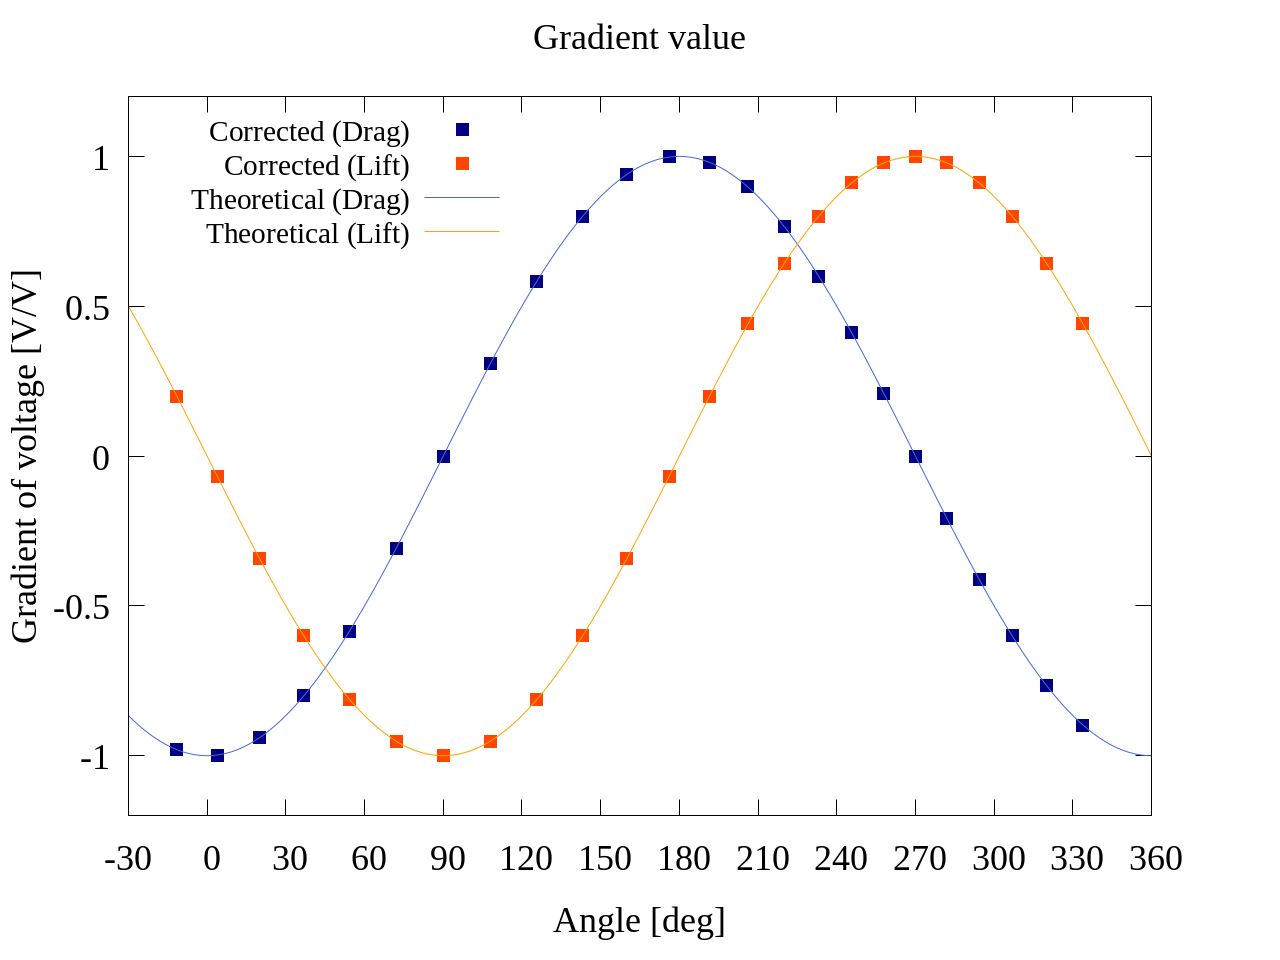
\includegraphics[width=95mm]{../../02_workspace/result/offset_dx=5.0_dy=0.0/plot/21/21-2_summary_offset.png}
    \caption{Corrected gradient [Case 4]}
  \end{center}
\end{figure}


Fig.17をみると算出された補正値は理論曲線上に位置していることがわかる.
しかし,プロットされているデータの角度は$\varphi$となるため,不等間隔となってしまうことがわかる.\par
また,Fig.18,Fig.19に,Case 5 および Case 6 におけるテストデータとその補正結果について示す.

\subsubsection{テストデータ : Case 5 ($\Delta x_\mathrm{test} = 5.0$ [mm],$\Delta x_\mathrm{test} = -5.0$ [mm])}
\begin{figure}[htbp]
  \begin{minipage}[b]{0.45\linewidth}
    \centering
    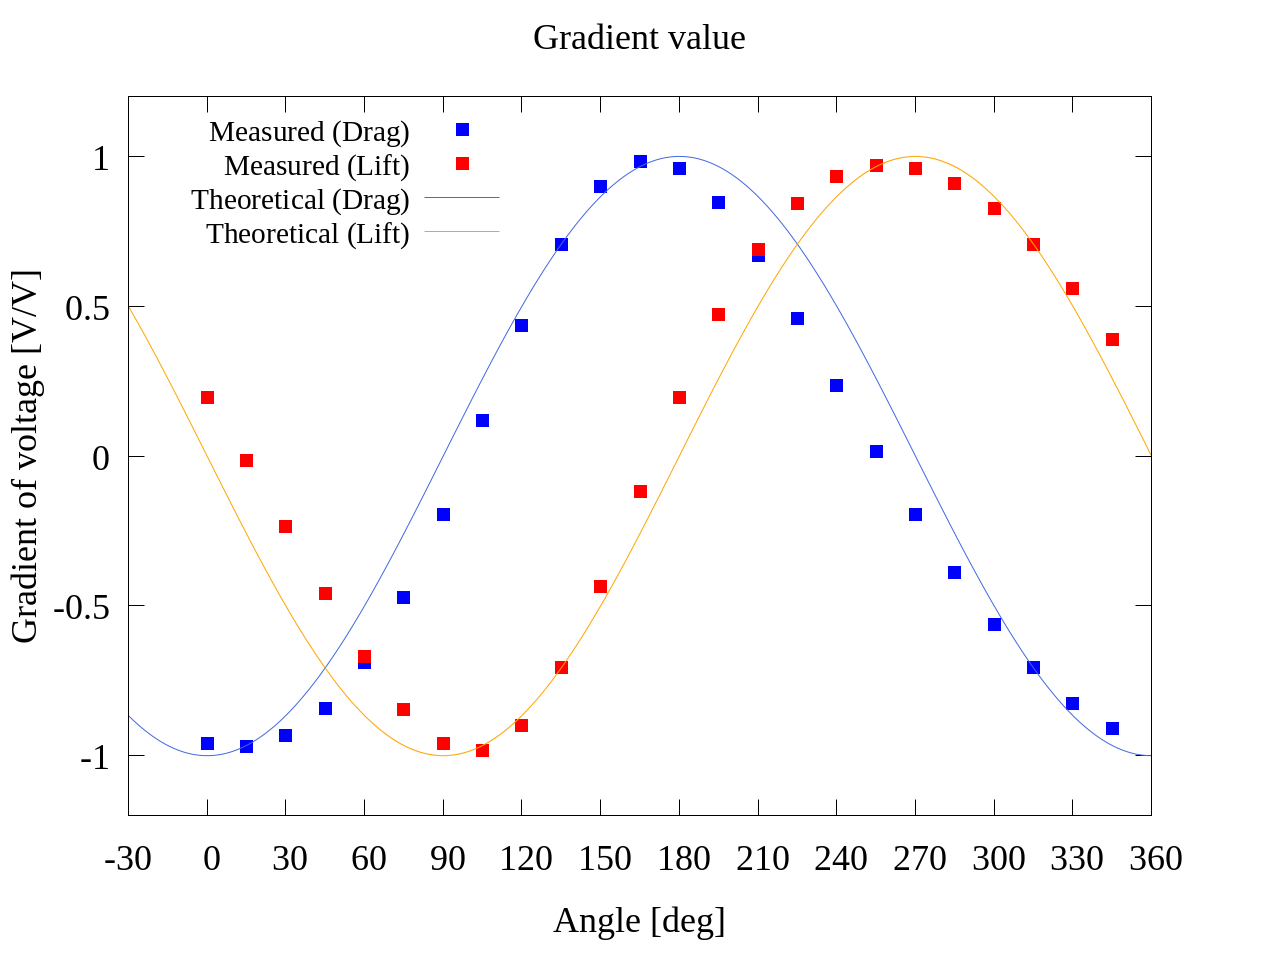
\includegraphics[width=65mm]{../../02_workspace/result/offset_dx=5.0_dy=-5.0/plot/20/20_adjust-value.png}
    \subcaption{Simulated gradient}
  \end{minipage}
  \begin{minipage}[b]{0.45\linewidth}
    \centering
    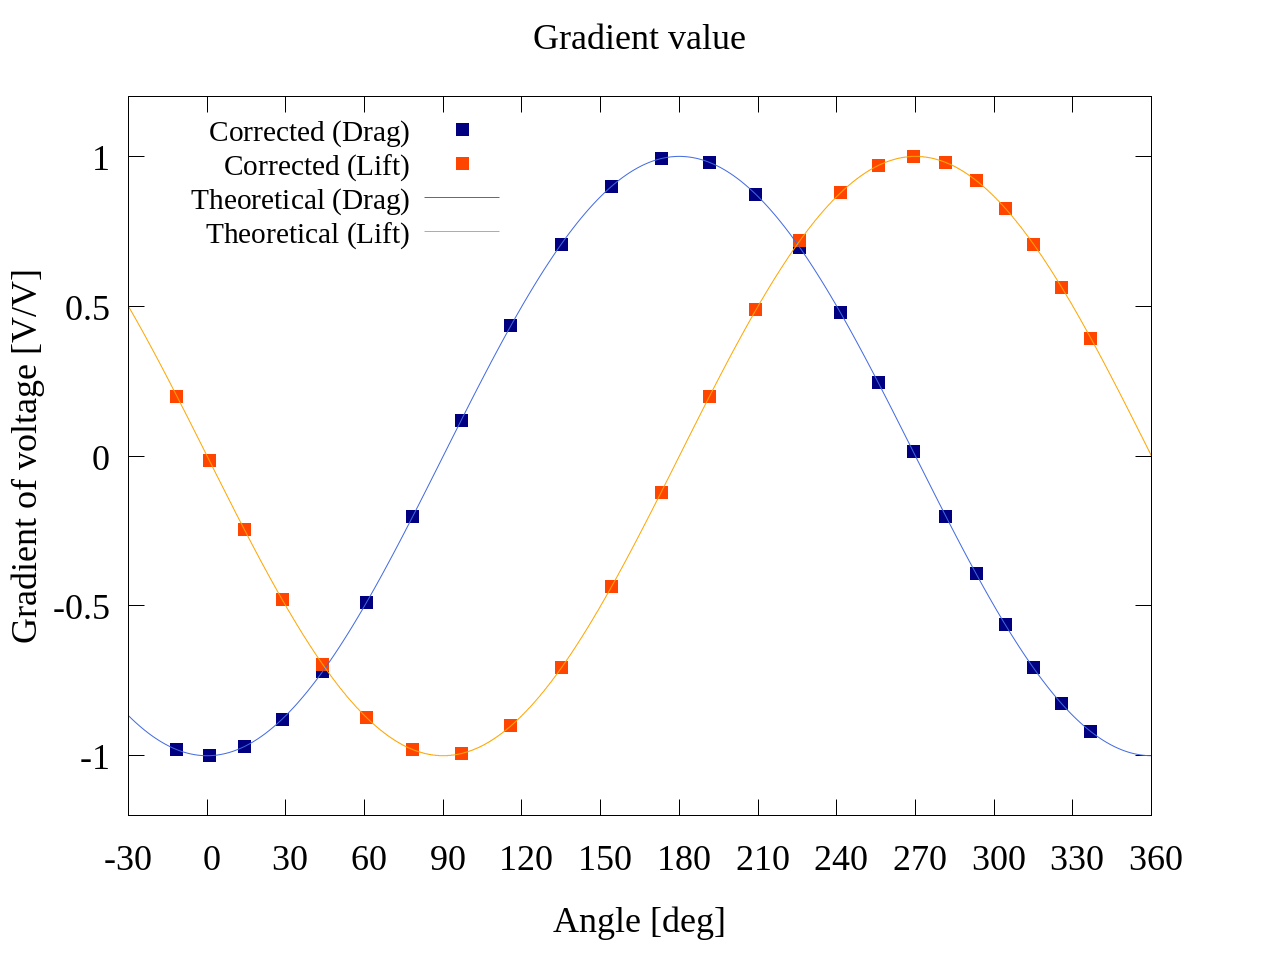
\includegraphics[width=65mm]{../../02_workspace/result/offset_dx=5.0_dy=-5.0/plot/21/21-2_summary_offset.png}
    \subcaption{Corrected gradient}
  \end{minipage}
  \caption{Teat data [Case 5]}
\end{figure}

\newpage

\subsubsection{テストデータ : Case 6 $\Delta x_\mathrm{test} = 10.0$ [mm],$\Delta x_\mathrm{test} = -5.0$ [mm]}
\begin{figure}[htbp]
  \begin{minipage}[b]{0.45\linewidth}
    \centering
    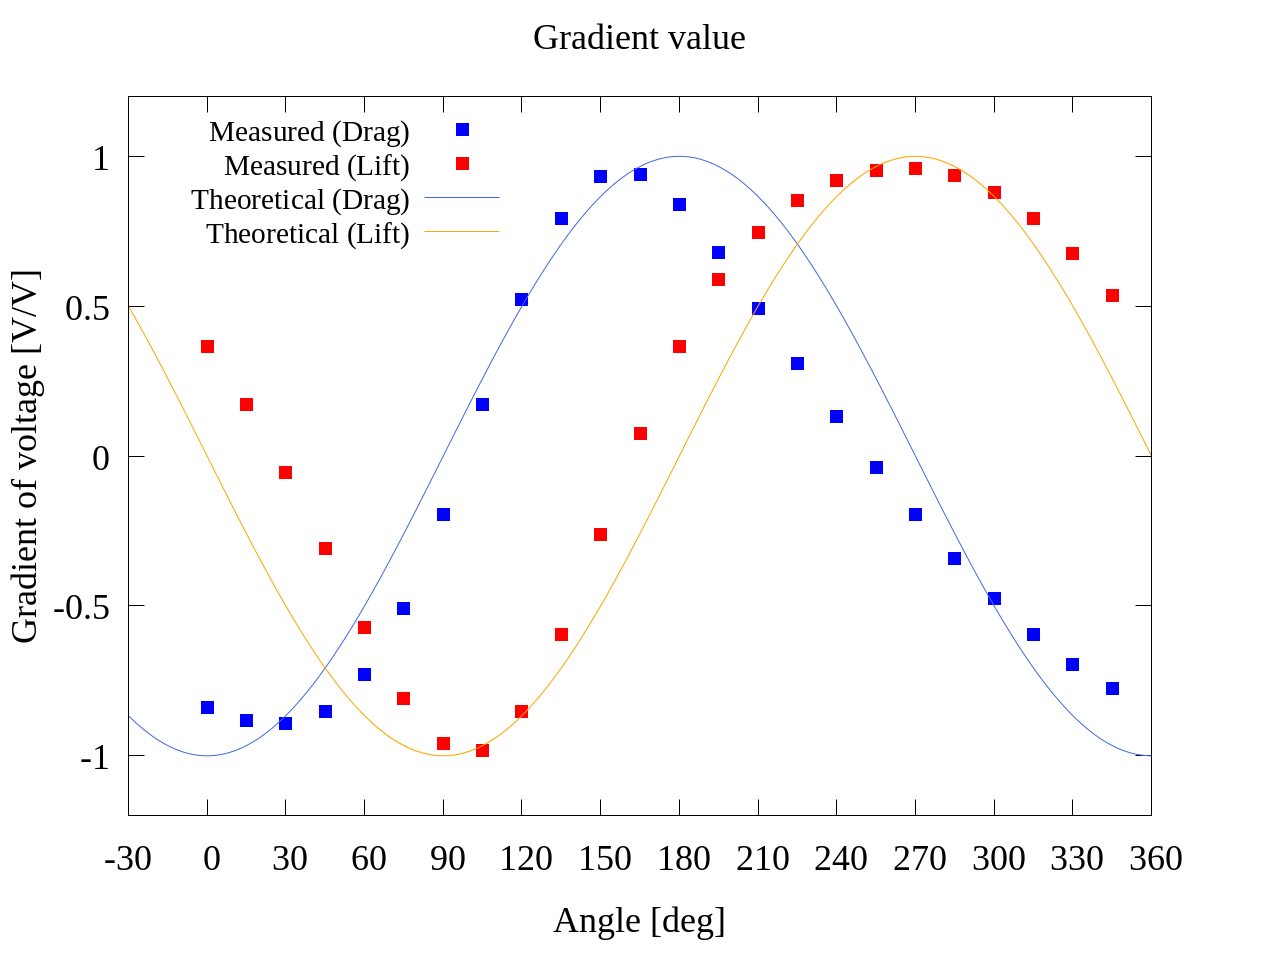
\includegraphics[width=65mm]{../../02_workspace/result/offset_dx=10.0_dy=-5.0/plot/20/20_adjust-value.png}
    \subcaption{Simulated gradient}
  \end{minipage}
  \begin{minipage}[b]{0.45\linewidth}
    \centering
    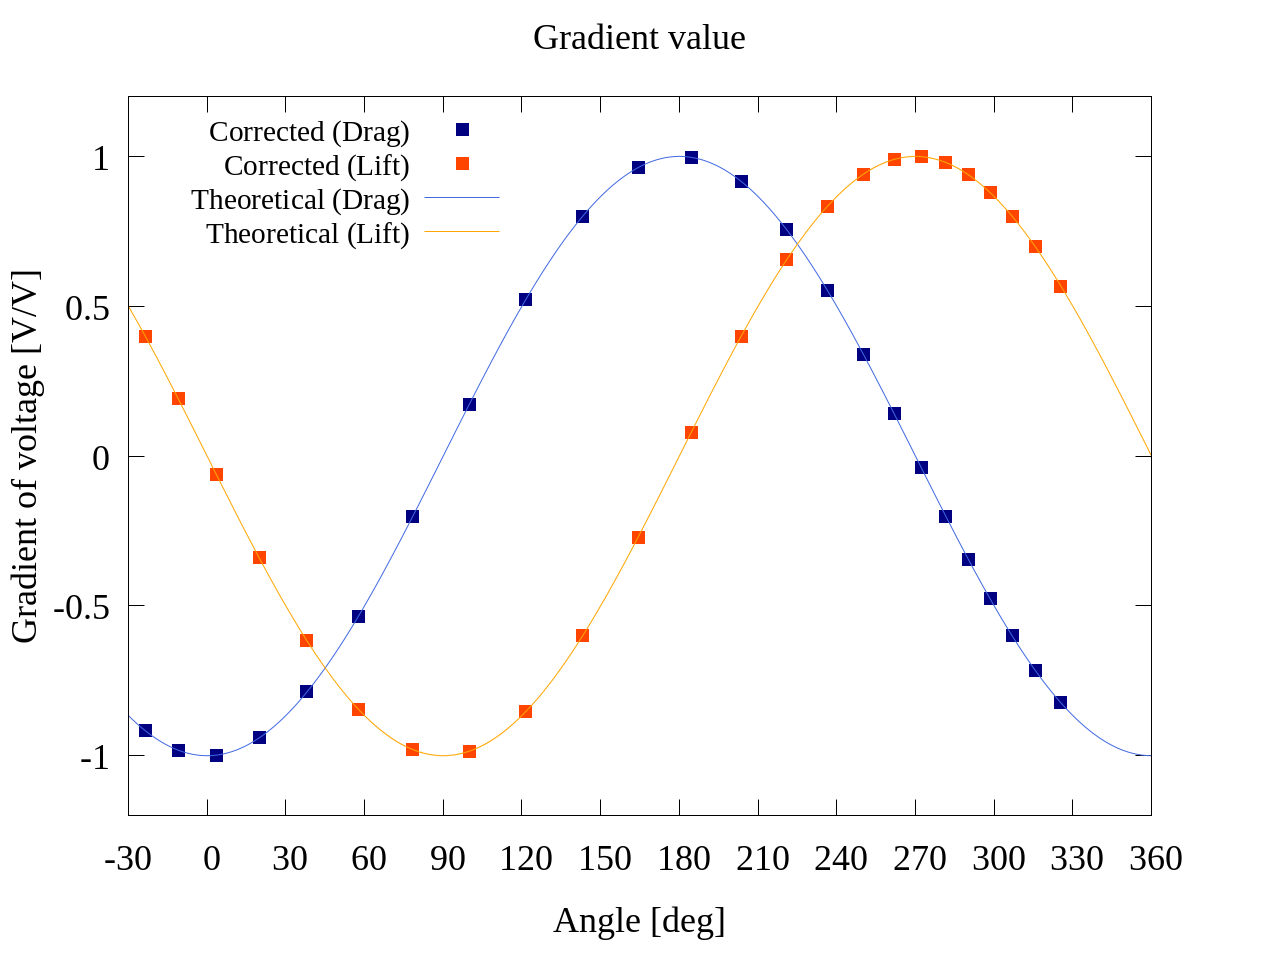
\includegraphics[width=65mm]{../../02_workspace/result/offset_dx=10.0_dy=-5.0/plot/21/21-2_summary_offset.png}
    \subcaption{Corrected gradient}
  \end{minipage}
  \caption{Teat data [Case 6]}
\end{figure}

\subsection{補正理論[3] : 複合状態における補正理論}

実際に校正実験を行う際には,座標系の回転,オフセットは同時に発生する.
したがって,上記の2つの補正理論を組み合わせて補正処理を行う必要がある.

\subsubsection{補正理論の適用順序}

構成した補正理論について,座標系の回転角$\theta_x$,$\theta_2$の特定の際に
離散フーリエ変換を適用することから,補正理論[2]を先に適用する必要がある.
また,上述のようにオフセットを考慮した場合,データ間隔が不等間隔となるため
回転角を特定するための離散フーリエ変換が適用できない.
したがって,ラグランジュ補間を用いて二次近似を行い,等間隔のデータを補完することとした.

\subsubsection{ラグランジュ補間}

一般にラグランジュ補間公式とは,$(x_1,f\left(x_1\right))$,$(x_2,f\left(x_2\right))$,
$(x_3,f \left(x_3\right))$,$\cdots$の点を通る関数$P\left(x\right)$を以下のように表す.

\begin{align}
  P\left(x\right)    & = \sum^{n+1}_{i=1} y_i \frac{f_i\left(x\right)}{f_i \left(x_i\right)} \\
  f_i \left(x\right) & = \prod_{k \neq i} \left(x - x_k\right)
\end{align}
\vskip \baselineskip

ここで,2次補間を行う場合,使用する3点を適切に選択する必要があるが
アルゴリズムを用いて処理を行いたい.
そこで,以下のような手順でデータを選択し,ラグランジュ補間を行った.

\subsubsection{使用するデータの選択}

校正実験では,15度ずつ測定しているため,計24点のデータを得ることができる.
補正理論[2]を用いた補正処理では,水槽座標系における作用力とその角度が算出される.
しかし,離散フーリエ変換を適用するとき,等間隔のデータが必要となるため15度ごとの補間値を算出しなければならない.
ここで,必要な補間値の角度を$\theta$とするとき,
実際の作用力の角度$\varphi$との差
$\delta \theta$を絶対値で評価することで,その値$|\delta \theta|$が
最も小さくなる角度$\varphi$とその前後のデータを使用することで,$\theta$に最も近い3点を選択することができる.

\begin{align}
  \delta \theta = |\theta - \varphi|
\end{align}
\vskip \baselineskip

\subsubsection{補正理論[3]のテストデータへの適用}
上述の補正理論より座標系の回転・オフセットを考慮したテストデータを構成する.
任意の回転角$\theta_{x\;\mathrm{test}}$,$\theta_{y\; \mathrm{test}}$,
任意のオフセット$\Delta x_\mathrm{test}$,$\Delta y_\mathrm{test}$を与え,
複合状態における出力電圧勾配について,$x''$軸方向を$v_{x''\;\mathrm{test}}$,
$y''$軸方向を$v_{y''\;\mathrm{test}}$とするとき,以下のように表される.
また,今回をTable 6のようなパラメータを用いてテストデータを構成した.

\begin{align}
  \theta                  & = \frac{\pi}{180} \; i \;\left(i = 0, 1, 2, 3, \cdots\right)                                                       \\
  \alpha                  & = \sin^{-1} \left( \frac{\Delta x_\mathrm{test} \sin \theta - \Delta y_\mathrm{test} \cos \theta}{r} \right)       \\
  \varphi                 & = \theta - \sin^{-1}\left(\frac{\Delta x_\mathrm{test} \sin \theta - \Delta y_\mathrm{test} \cos \theta}{r}\right) \\
  \notag                                                                                                                                       \\
  v_{x'' \;\mathrm{test}} & = - \cos \alpha \cos \left(\varphi - \theta_{x\; \mathrm{test}} \right)                                            \\
  v_{y'' \;\mathrm{test}} & = - \cos \alpha \sin \left(\varphi - \theta_{y\; \mathrm{test}}\right)
\end{align}

\begin{table}[htbp]
  \begin{center}
    \caption{Test data conditions (3)}
    \begin{tabular}{|p{30mm}|p{20mm}|p{20mm}|p{20mm}|p{20mm}|}
      \hline
      \multicolumn{1}{|c|}{}       & \multicolumn{1}{|c|}{$\theta_{x\;\mathrm{test}}$ [deg]} & \multicolumn{1}{|c|}{$\theta_{y\;\mathrm{test}}$ [deg]} & \multicolumn{1}{|c|}{$\Delta x_\mathrm{test}$ [mm]} & \multicolumn{1}{|c|}{$\Delta y_\mathrm{test}$ [mm]} \\ \hline
      \multicolumn{1}{|c|}{Case 7} & \multicolumn{1}{|c|}{10.0}                              & \multicolumn{1}{|c|}{-5.0}                              & \multicolumn{1}{|c|}{5.00}                          & \multicolumn{1}{|c|}{-2.50}                         \\ \hline
    \end{tabular}
  \end{center}
\end{table}

\newpage

Case 7 に対する座標系の回転おける補正理論の適用過程について説明する.
はじめに,構成したテストデータをFig.20 に示す.
また,補正理論[2]を適用した結果をFig.21 に示す.

\begin{figure}[htbp]
  \begin{center}
    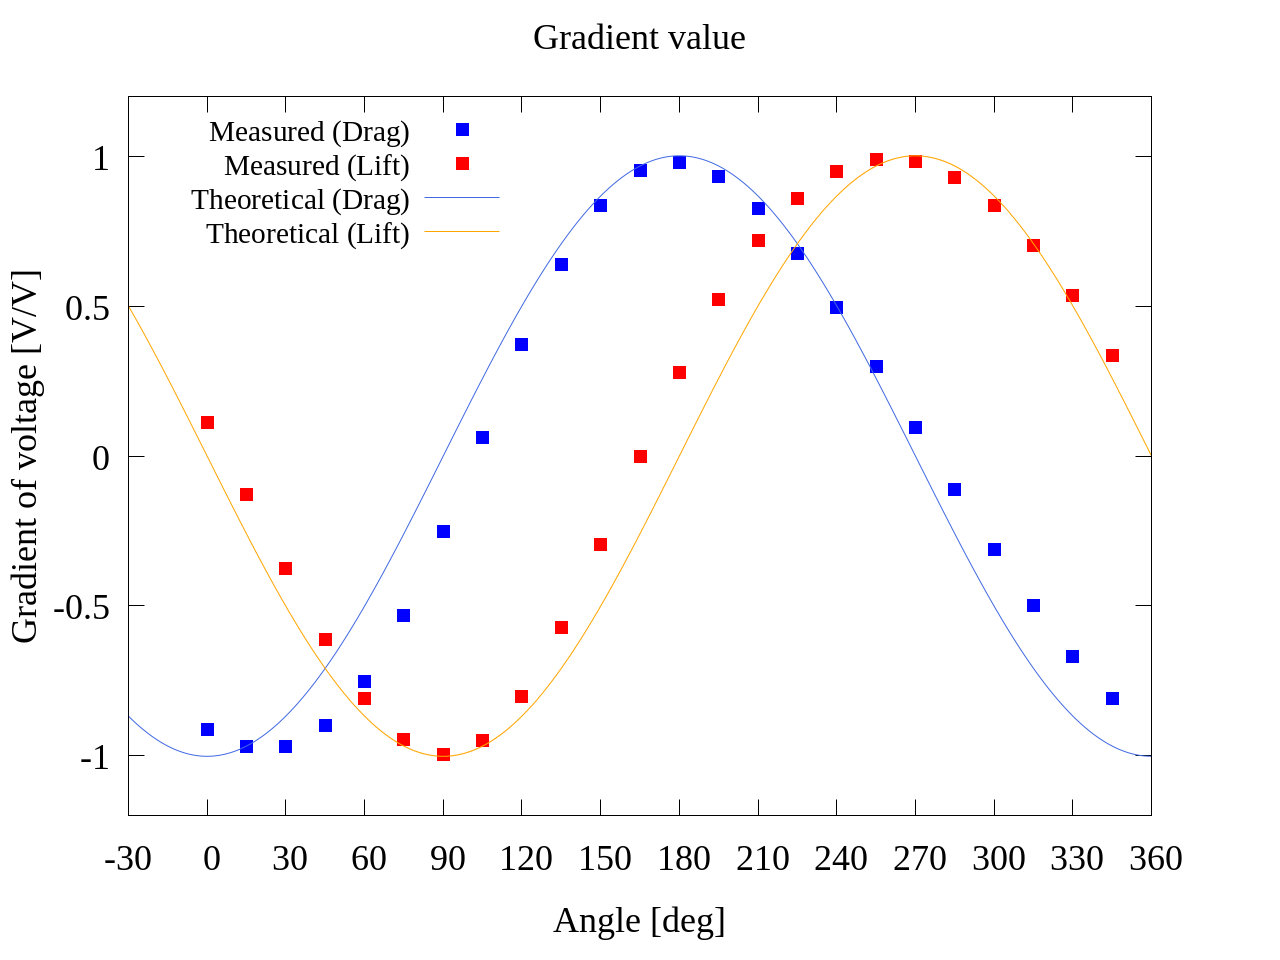
\includegraphics[width=95mm]{../../02_workspace/result/simulation_tx=10.0_ty=-5.0_dx=5.00_dy=-2.50/plot/20/20_adjust-value.png}
    \caption{Simulated gradient [Case 7]}
    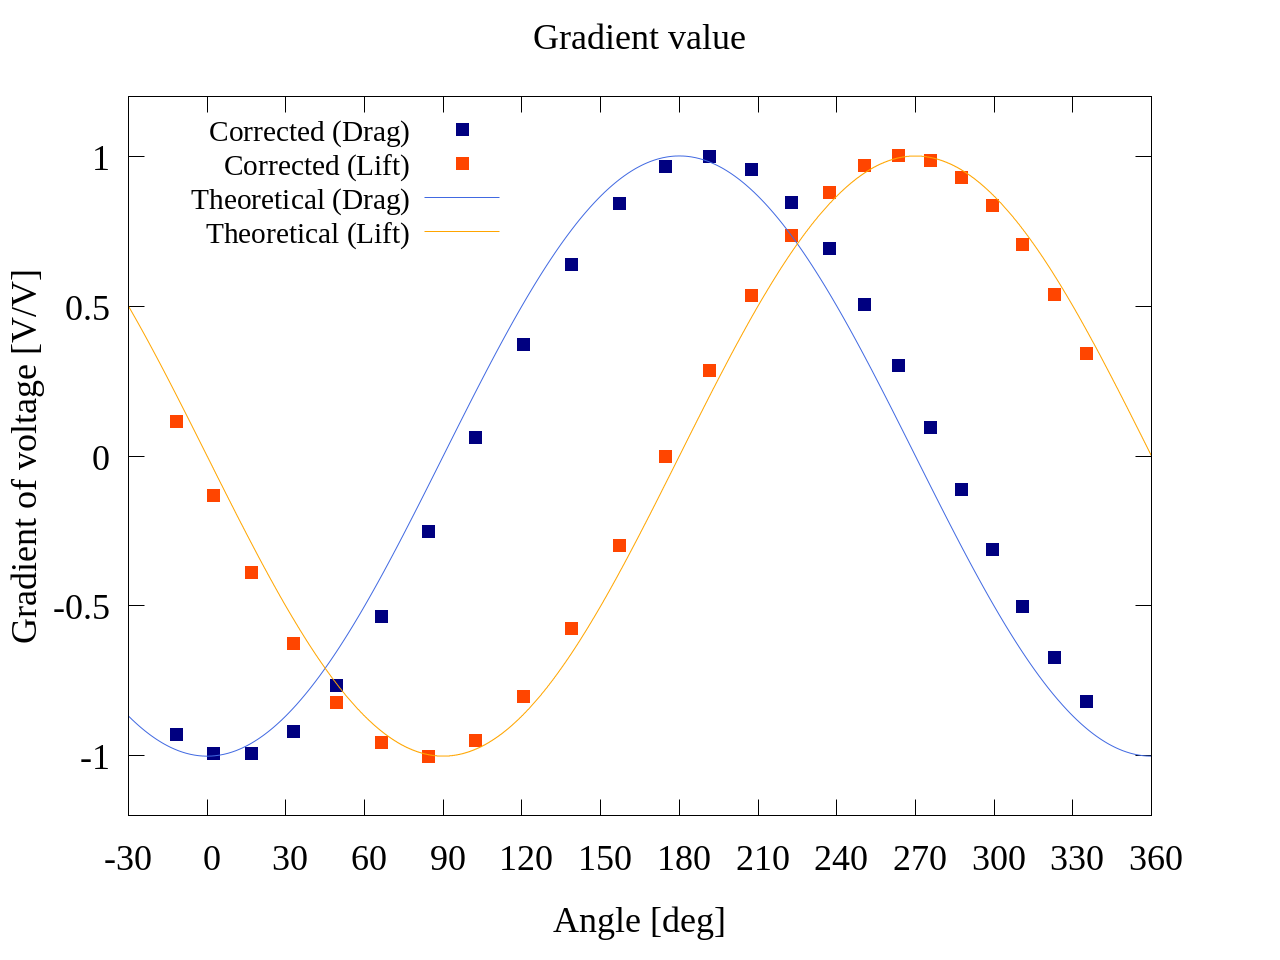
\includegraphics[width=95mm]{../../02_workspace/result/simulation_tx=10.0_ty=-5.0_dx=5.00_dy=-2.50/plot/21/21-2_summary_offset.png}
    \caption{Offset Corrected gradient [Case 7]}
  \end{center}
\end{figure}

\newpage

理論曲線と比較して,波形の再現はされているが,位相差があるようにみえる.
また,プロットされたデータ間隔は異なることもわかる.
このとき,ラグランジュ補間を用いて,等間隔のデータを得るための処理を行う.
なお,データの採用点については上述の処理によって行うこととする.
ラグランジュ補間を行った結果をFig.22に示す.

\begin{figure}[htbp]
  \begin{center}
    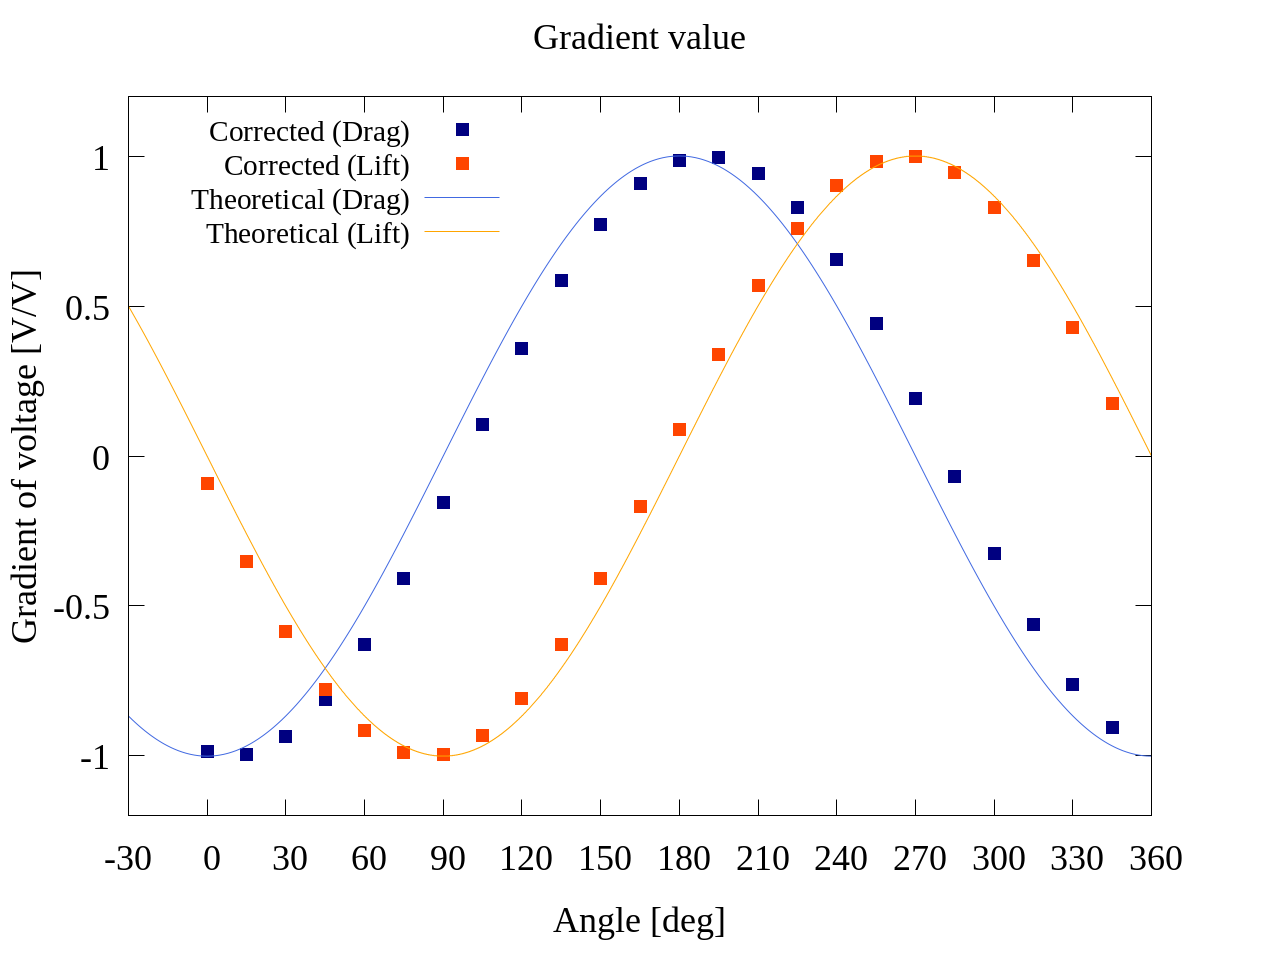
\includegraphics[width=95mm]{../../02_workspace/result/simulation_tx=10.0_ty=-5.0_dx=5.00_dy=-2.50/plot/21/21-3_summary_interpolated.png}
    \caption{Interpolated data [Case 7]}
  \end{center}
\end{figure}

上記のFig.20,Fig.21と比較するとFig.22は等間隔のデータを得られていることがわかる.
次に,フーリエ変換を適用する.
このときの結果をFig.23に示す.
また,波数1の成分についての算出値をTable 7に示す.

\begin{figure}[htbp]
  \begin{minipage}[b]{0.45\linewidth}
    \centering
    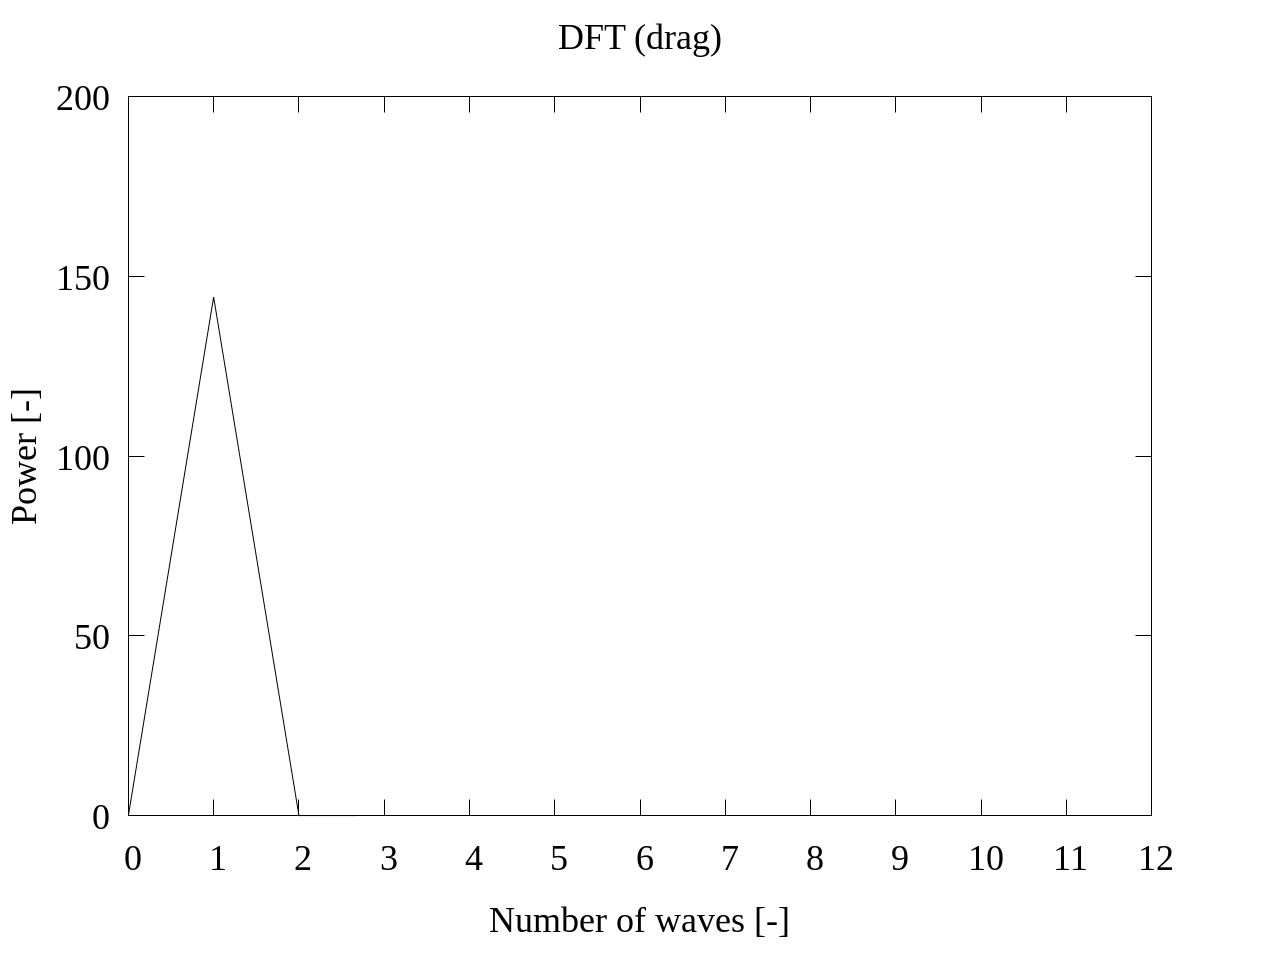
\includegraphics[width=65mm]{../../02_workspace/result/simulation_tx=10.0_ty=-5.0_dx=5.00_dy=-2.50/plot/07/07-3_dft-drag.png}
    \subcaption{Drag}
  \end{minipage}
  \begin{minipage}[b]{0.45\linewidth}
    \centering
    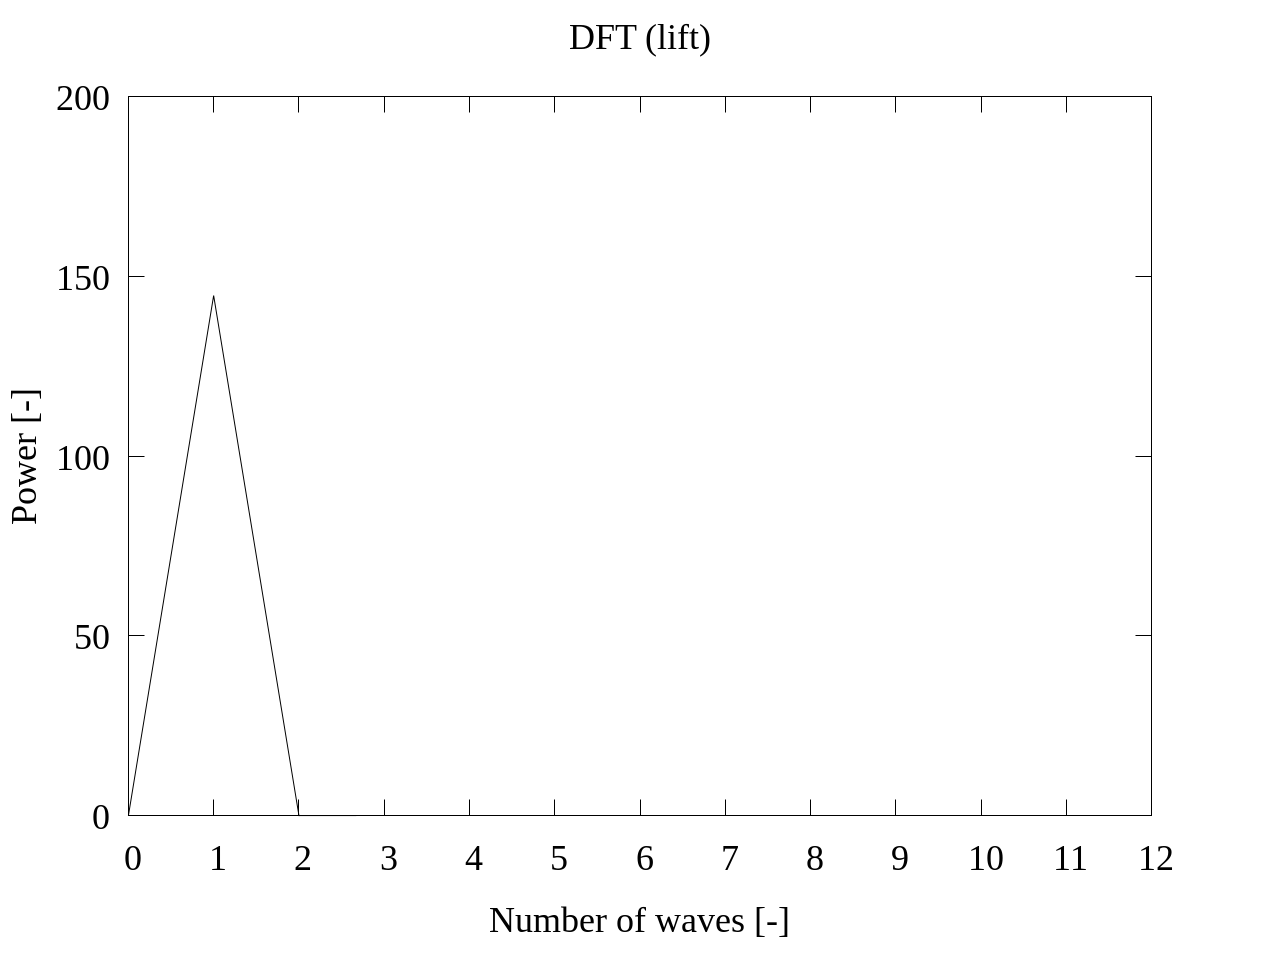
\includegraphics[width=65mm]{../../02_workspace/result/simulation_tx=10.0_ty=-5.0_dx=5.00_dy=-2.50/plot/07/07-4_dft-lift.png}
    \subcaption{Lift}
  \end{minipage}
  \caption{DFT spectrum [Case 7]}
\end{figure}

\begin{table}[htbp]
  \begin{center}
    \caption{DFT result value [Case 7]}
    \begin{tabular}{|p{30mm}|p{20mm}|p{20mm}|}
      \hline
      \multicolumn{1}{|c|}{}     & \multicolumn{1}{|c|}{Re}      & \multicolumn{1}{|c|}{Im}     \\ \hline
      \multicolumn{1}{|c|}{Drag} & \multicolumn{1}{|c|}{-11.835} & \multicolumn{1}{|c|}{2.083}  \\ \hline
      \multicolumn{1}{|c|}{Lift} & \multicolumn{1}{|c|}{-1.081}  & \multicolumn{1}{|c|}{11.978} \\ \hline
    \end{tabular}
  \end{center}
\end{table}

\newpage
Fig.23より,波数1についてピークがあることがわかり,
座標軸の回転における補正理論の適用結果と同様にデータの特徴を正しく捉えられているといえる.
ここで,Table 7について,式(5),式(6),式(7)より
回転角$\theta_x$,$\theta_y$をそれぞれ算出し,その値をTable 8に示す.

\begin{table}[htbp]
  \begin{center}
    \caption{Specified rotation angle [Case 7]}
    \begin{tabular}{|p{30mm}|p{20mm}|p{20mm}|}
      \hline
      \multicolumn{1}{|c|}{}       & \multicolumn{1}{|c|}{$\theta_x$ [deg]} & \multicolumn{1}{|c|}{$\theta_y$ [deg]} \\ \hline
      \multicolumn{1}{|c|}{Case 7} & \multicolumn{1}{|c|}{10.018}           & \multicolumn{1}{|c|}{-5.158}           \\ \hline
    \end{tabular}
  \end{center}
\end{table}


結果より,算出された回転角$\theta_{x\;\mathrm{test}}$,$\theta_{y\;\mathrm{test}}$は
Table 8の Case 7 で設定したパラメータと比較すると,異なっていることがわかる.
これは,ラグランジュ補間公式を用いた2次近似による誤差が生じているためと考えられる.

また,算出した回転角$\theta_{x\;\mathrm{test}}$,$\theta_{y\;\mathrm{test}}$を用いて
補正理論[1]を適用した結果をFig.24に示す.

\begin{figure}[htbp]
  \begin{center}
    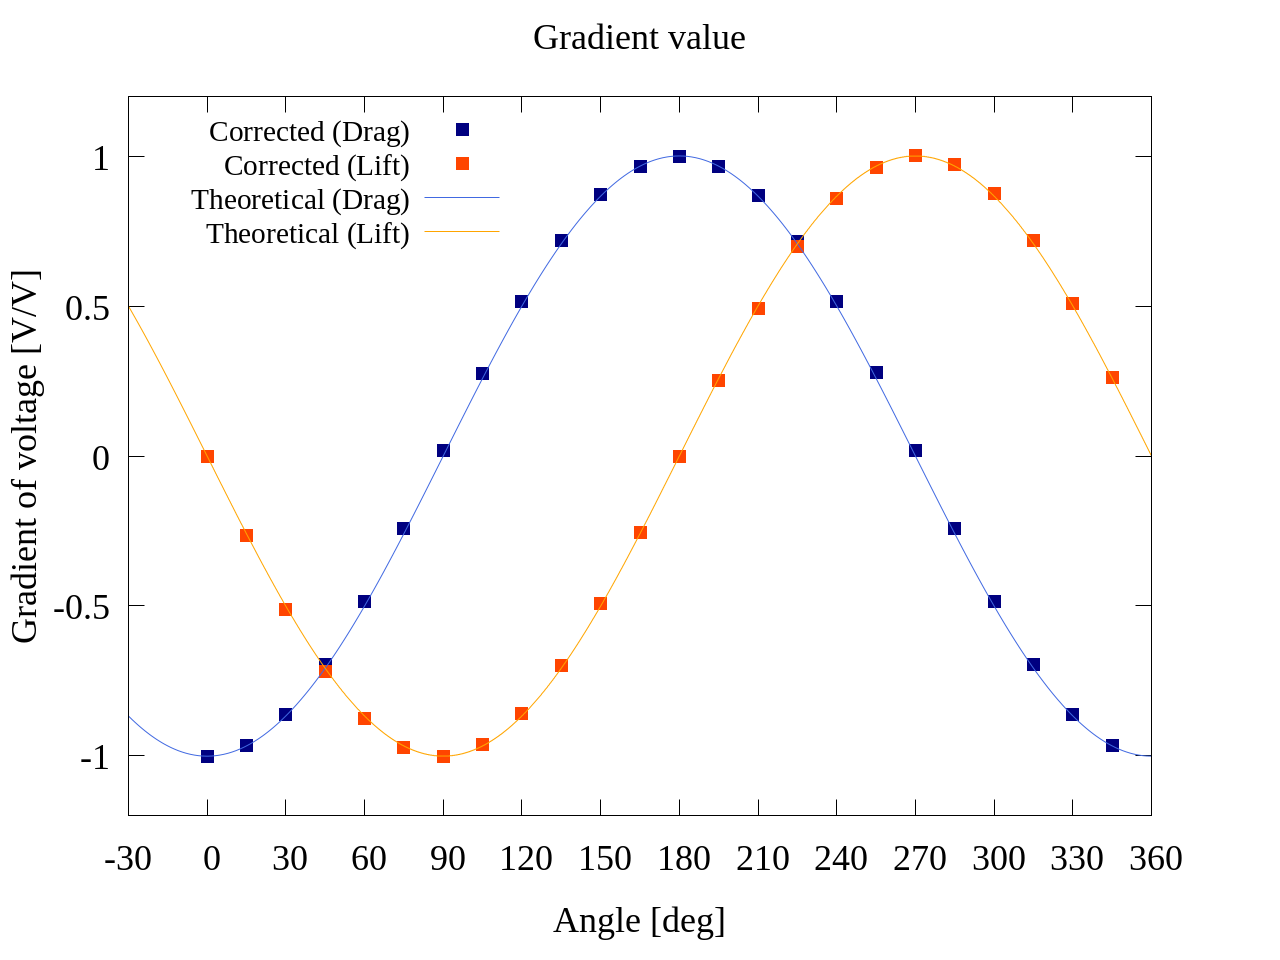
\includegraphics[width=95mm]{../../02_workspace/result/simulation_tx=10.0_ty=-5.0_dx=5.00_dy=-2.50/plot/21/21-4_summary.png}
    \caption{Corrected gradient [Case 7]}
  \end{center}
\end{figure}

Fig.24をみると,理論曲線と補正値がおおよそ一致していることが考えられる.

\subsection{正味出力電圧勾配による評価}

また,補正適用後に得られる水槽座標系の出力電圧$v_x$,$v_y$から,
以下の式によって正味出力電圧勾配$v_{\mathrm{net}}$と定義し,
その結果をFig.25に示す.

\begin{align}
  v_{\mathrm{net}} & = \sqrt{v_x^2 + v_y^2}
\end{align}

\begin{figure}[htbp]
  \begin{center}
    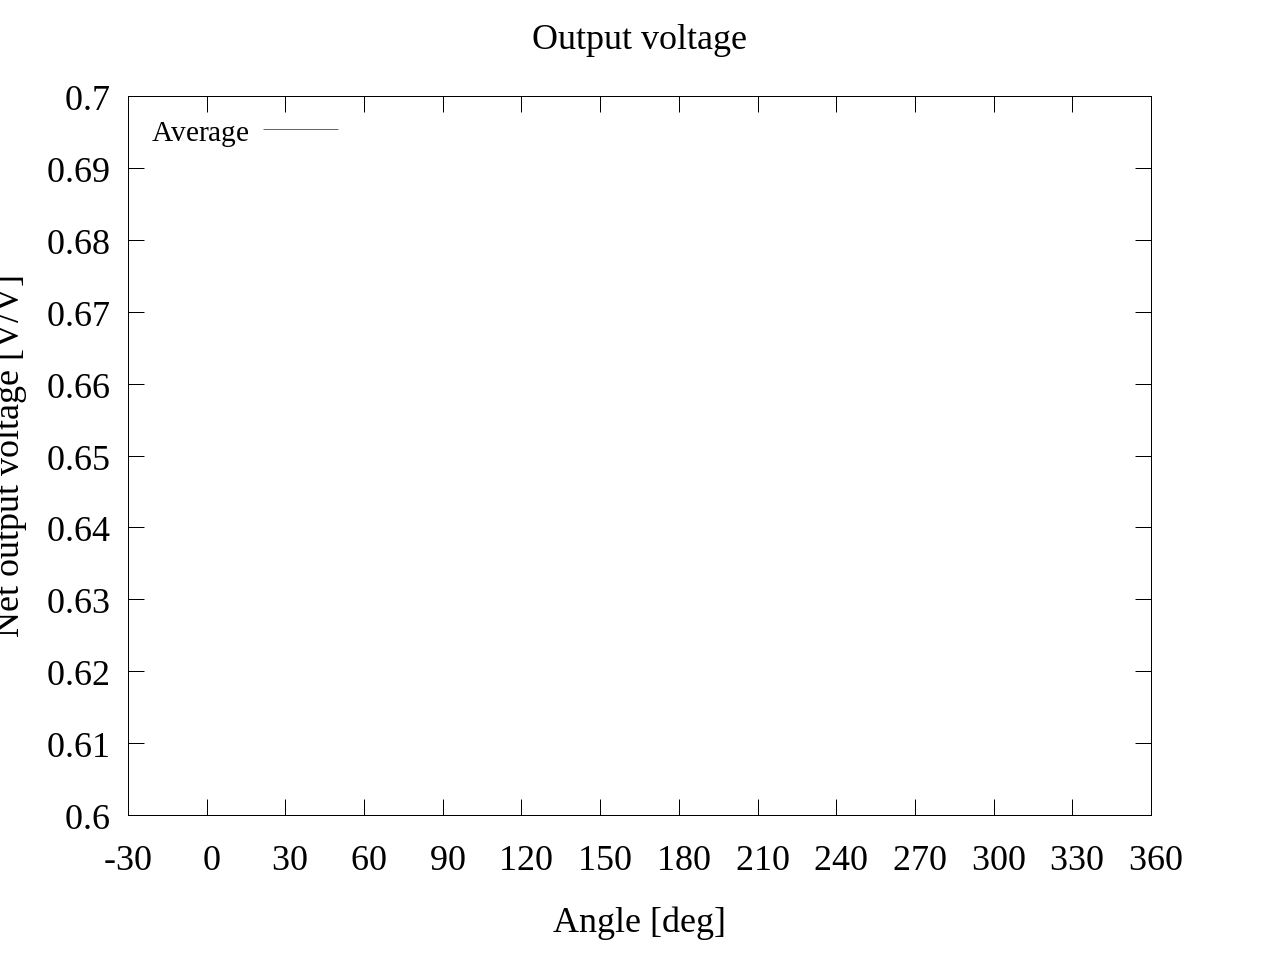
\includegraphics[width=95mm]{../../02_workspace/result/simulation_tx=10.0_ty=-5.0_dx=5.00_dy=-2.50/plot/09/09_summary-outputvoltage-net.png}
    \caption{Net voltage gradient [Case 7]}
  \end{center}
\end{figure}

Fig.25をみると,テストデータ[Case 7]における正味出力電圧はおおよそ一定になることがわかる.
同時に,細かな変動もみられるが,これはラグランジュ補間による誤差の影響であると考えられる.

以上より,構成した補正理論は正しく機能しているといえ,
座標系の回転,座標系のオフセット距離が存在する場合であっても,
オフセット距離が既知である場合,処理を行う過程の中で
座標系の回転角$\theta_x$,$\theta_y$を推定し,
水槽座標系における出力電圧を推定することができるといえる.

\newpage